
\section{Considerações Iniciais}

Neste capítulo, são apresentados e discutidos os conceitos fundamentais para o entendimento desta tese. Está organizado da seguinte forma: na Seção~\ref{Cap2_Sec2_Desenvolvimento_Dirigido_a_Modelos}, os conceitos sobre Engenharia Dirigido por Modelos são salientados; na Seção~\ref{sec:refatoracao}, são definidos os conceitos sobre refatoração, bem como refatorações para modelos. Na Seção~\ref{sec:modernizacaoOrientada_Arquitetura}, é feita uma contextualização sobre a Modernização Dirigida a Arquitetura; na Seção~\ref{sec:knowledge_discovery_meta_model}, o metamodelo KDM é apresentado; na Subseção~\ref{subsection:codePackage}, é descrito o pacote \texttt{Code}; na Subseção~\ref{sec:actionPackage}, é descrito o pacote \texttt{Action}; na Subseção~\ref{sec:structurePackage}, é apresentado o pacote \texttt{Structure}; na Seção~\ref{sec:Ferramenta_de_apoio_KDM_capitulo}, é mostrada uma ferramenta de apoio ao KDM; na Seção~\ref{capitulobaclCOnsideracoesFinais}, as considerações finais deste capítulo são destacadas.

\section{Engenharia Dirigida por Modelos}\label{Cap2_Sec2_Desenvolvimento_Dirigido_a_Modelos}

De acordo com~\citeonline{Booch:2004:OAD:975416} modelos são abstrações de sistemas que permitem raciocinar e entender o sistema, ignorando detalhes irrelevantes, enquanto o foco é dado aos detalhes mais relevantes. Segundo~\citeonline{Brown_2007, Bezivin02apreliminary}, a utilização de modelos para o desenvolvimento de software não é algo novo. Modelos são usados há algumas décadas para auxiliar a concepção e o projeto de software, sendo utilizados basicamente nas fases iniciais do desenvolvimento. Por exemplo, modelos como os da UML~\cite{UML:OMG} não fazem parte do software em si, embora sejam importantes para o entendimento e a construção. Os desenvolvedores os criam, mas os descartam, implementando as funções de forma manual e realizando manutenções somente no código-fonte. Desse modo, o conhecimento acerca da solução fica criptografado no código-fonte e dificilmente é reutilizado. Portanto, há necessidade de criar modelos que representem esse conhecimento e que possam ser úteis tanto para a documentação, quanto para a construção e manutenção de software.


A partir dessa ideia, a \textit{Model-Driven Engineering} (MDE) surge como uma solução complementar aos processos de desenvolvimento tradicionais~\cite{Lima_2007}. A MDE é uma abordagem que propõe reduzir a distância semântica entre o problema do domínio e a solução/implementação. Nessa abordagem, o desenvolvimento de software ocorre por meio de modelos que protegem os desenvolvedores das complexidades da implementação e de transformações que originam o código-fonte de maneira automatizada a partir das informações contidas nesses modelos. Na literatura, é possível também identificar MDE como outros acrônimos, por exemplo, \sigla{MDD}{\textit{Model-Driven Development}}, \sigla{MDSD}{\textit{Model-Driven Software Development}} ou MD*~\cite{Kleppe:2003}, e todos eles dizem respeito à mesma abordagem. O que é importante ter em mente sobre MDE é que modelos são utilizados no centro do processo de desenvolvimento e manutenção de software. Na MDE, os modelos assumem o papel principal em todo o ciclo de vida de um software e a relevância dos modelos vai além da documentação do software desenvolvido. Na MDE, modelos passam a ser utilizados como artefatos principais; eles podem ser compreendidos por computadores e são fundamentais para o desenvolvimento do software, pois podem ser manipulados, refinados e transformados em uma nova versão, até que a partir deles seja gerado o código-fonte~\cite{Kleppe:2003, Brown_2007, Ben_Ammar}.

Na MDE, o enfoque do desenvolvimento é direcionado aos modelos, ou seja, a modelagem deixa de ser meramente uma forma de planejar o código e passa a ser uma forma de construir o software. O nível de abstração da programação torna-se mais elevado, reduzindo a necessidade do desenvolvedor de interagir manualmente com o código-fonte~\cite{Braganca_Machado}. É importante salientar que a MDE não tem como objetivo substituir o processo tradicional de desenvolvimento de software~\cite{Kleppe:2003, Brown_2007, Braganca_Machado} e sim contribuir para o seu aprimoramento. O OMG~\cite{ADM:OMG} definiu um modelo de arquitetura para o MDE, conhecido como \emph{Model-Driven Architecture} (MDA), o qual tem como objetivo promover o uso de modelos no desenvolvimento de software, para fornecer uma solução ao gerenciamento da complexidade do desenvolvimento, manutenção e evolução de sistemas de software e favorecer a interoperabilidade e portabilidade desses sistemas.

O OMG definiu formalmente a MDA como uma abordagem que é bem definida pela ideia de separar a especificação das operações de um sistema dos detalhes de como tal sistema usa as potencialidades de sua plataforma. Isso possibilita que ferramentas ofereçam a especificação de um sistema de forma independente de plataforma. De acordo com o OMG, os principais objetivos da MDA são a portabilidade, a interoperabilidade e a reusabilidade. Para alcançar esses objetivos a MDA divide o desenvolvimento de software em níveis de abstração~\cite{France_2007, Ben_Ammar}:

\begin{itemize}
	\item Modelo Independente de Computação (do inglês - \sigla{CIM}{\emph{Computation Independent Model}}): descreve o negócio, ou ambiente, no qual o software irá operar. Como a decisão a respeito da informatização é feita por uma pessoa e não por uma ferramenta de transformação, dificilmente a transformação automatizada desse modelo para o de nível seguinte é implementada;
	\item Modelo Independente de Plataforma (do inglês - \sigla{PIM}{\emph{Platform Independent Model}}): nível de análise em que ocorre a definição das características do software ou domínio. Esse modelo pode ser transformado para um ou mais modelos do nível seguinte;
	\item Modelo Específico de Plataforma (do inglês - \sigla{PSM}{\textit{Platform Specific Model}}): nível de projeto que considera as tecnologias de implementação, devendo existir uma instância desse modelo para cada plataforma de implantação do software. A partir desse modelo ocorre a transformação para o código-fonte.
\end{itemize}

Com base nos princípios mencionados, podem-se citar as seguintes vantagens da MD*~\cite{Hutchinson_2011, France_2007, Schmidt_2006}:

\begin{enumerate}
	\item Maior facilidade na criação dos modelos das aplicações, pois é utilizada uma linguagem específica para o domínio do problema;
	\item Maior produtividade e redução do esforço dos desenvolvedores, pois a maior parte do código-fonte das aplicações pode ser gerado a partir dos modelos;
	\item Maximização do tempo de vida útil dos modelos e de outros artefatos, pois, como são necessários para a geração de código, eles são menos propensos a serem descartados pelos desenvolvedores nos processos de manutenção;
	\item Flexibilidade de desenvolvimento, pois os modelos independentes de plataforma armazenam a lógica do sistema e são menos sensíveis a mudanças;
	\item O conhecimento a respeito do software não fica exclusivamente na mente dos desenvolvedores e no código, fazendo com que os processos de desenvolvimento e de manutenção fiquem menos vulneráveis às oscilações de pessoal.
\end{enumerate}

A MD* não pretende substituir os processos tradicionais de desenvolvimento de software, e sim contribuir para seu aprimoramento de uma maneira racional para mover informações de uma fase de desenvolvimento para outra, trazendo respostas rápidas e eficientes para atender as necessidades inesperadas de novos requisitos.

De acordo com~\citeonline{Kleppe:2003}, um modelo deve ser definido como uma descrição de um (ou de uma parte) sistema expresso em uma linguagem bem definida, isto é, respeitando uma sintaxe e uma semântica. Essa descrição deve ser conveniente para uma interpretação automatizada por computadores. Assim, para criar um modelo, deve-se seguir uma sintaxe precisa e uma semântica bem definida a fim de regulamentar a criação de elementos e suas relações. Em MDE, esse formalismo pode ser alcançado utilizando uma linguagem de modelagem. Tais linguagens são especificações que contêm os elementos bases para construir modelos, concebidas dentro de um domínio limitado e com objetivos específicos. Usualmente, uma linguagem de modelagem pode ser gráfica ou textual com notação matemática e deve permitir a definição de modelos sem ambiguidades. O uso de uma linguagem bem definida sintaticamente e semanticamente permite o entendimento e manipulação de modelos por pessoas e computações~\cite{Hutchinson_2011, France_2007, Schmidt_2006}.

Uma linguagem de modelagem geralmente está em conformidade com um metamodelo. Um metamodelo é um modelo que define uma linguagem para representar um modelo. A linguagem de modelagem é simplesmente um modelo do metamodelo. Ela define a estrutura, a semântica e as restrições para uma família de modelos~\cite{Mellor_2004}. Na Figura~\ref{fig:metamodelosCamadas}, são apresentados os quatro níveis de modelos da MDE. É importante notar que as relações entre os níveis descritos na Figura~\ref{fig:metamodelosCamadas} são do tipo \aspas{\texttt{instance of}} (instância de), definido por~\citeonline{Bezivin02apreliminary, Brambilla_2012}. Os quatros níveis são descritos a seguir: 

\begin{figure}[htb]
 \caption{Arquitetura de Metamodelagem.}
 \label{fig:metamodelosCamadas}
 \centering
 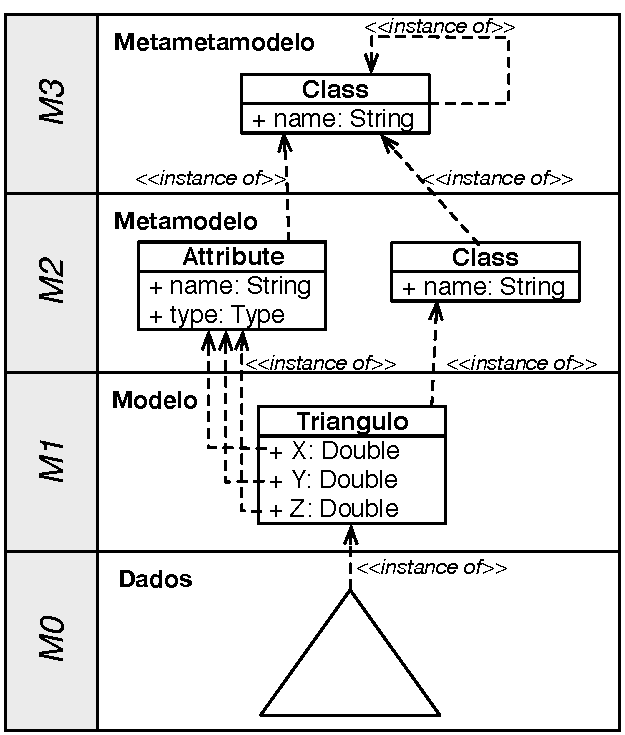
\includegraphics[scale=0.9]{images/Arquitetura_de_metamodelagem}
 \fautor
\end{figure}

\begin{itemize}
	\item metametamodelo (M3): M3 constitui a base da arquitetura de meta-modelagem. A função primordial desse nível é definir linguagens para especificar metamodelos. Um meta-metamodelo define um modelo de mais alto nível de abstração que o metamodelo, e o primeiro é tipicamente mais compacto que o segundo. \textit{Meta-Object Facility} (MOF)~\cite{MOF} e \sigla{EMF}{\emph{Eclipse-Modeling Framework}}\cite{EMF} são exemplos de metametamodelos;
	\item metamodelo (M2): um metamodelo representa uma instância de um metametamodelo. A função principal do nível do metamodelo é definir uma linguagem para especificar modelos. Os metamodelos são tipicamente mais elaborados que os metametamodelos. Por exemplo, a UML~\cite{UML:OMG} e o KDM~\cite{KDM:ISO} possuem metamodelos que os descrevem estruturalmente;
	\item modelo (M1): um modelo é uma instância de um metamodelo. A função principal do nível de modelo é definir uma linguagem para descrever um domínio específico;
	\item dados (M0): os objetos de usuários representam os dados finais. A principal responsabilidade dos objetos de usuários é descrever um domínio específico em uma plataforma final.
\end{itemize}

Um objetivo claro da MDA é fornecer um \textit{framework} que integra os padrões existentes do OMG. Os principais padrões do OMG utilizados nesta tese são:

\begin{itemize}
\item \textit{Meta Object Facility} (MOF): Linguagem abstrata e um \textit{framework} para especificação, construção e gerenciamento de metamodelos independentes de plataforma. Essa especificação contém um conjunto de construtores que é utilizado para a definição de metamodelos. MOF pode ser utilizado para definir outras linguagens;
\item \sigla{UML}{\textit{Unified Modeling Language}}: Linguagem para especificação, construção, visualização e documentação de artefatos de software. Essa linguagem permite a modelagem de diferentes aspectos ou pontos de vista de um sistema;
\item \textit{Knowledge Discovery Metamodel} (KDM): Metamodelo utilizado para representar em nível de modelos artefatos de sistemas de software. Na Seção~\ref{sec:knowledge_discovery_meta_model}, maiores informações sobre esse metamodelo, bem como suas metaclasses são apresentadas;
\item \textit{XML Metadata Interchange} (XMI): Padrão do OMG para troca de informação baseado em \sigla{XML}{\textit{eXtensible Markup Language}}. Pode ser utilizado para trocar qualquer informação, cujo metamodelo pode ser expresso utilizando MOF. O uso mais comum da XMI é como um formato de intercâmbio de modelos UML, embora também possa ser utilizado para a serialização de modelos de outras linguagens;
\item \textit{ATL Transformation Language} (ATL): Implementação da \textit{Query/View/Transformation} (QVT) que é uma especificação híbrida padronizada para transformação de modelos no contexto de metamodelagem MOF. ATL aceita construções declarativas e imperativas (ver Subseção~\ref{sub:atl_transformation_language});
\sigla{OCL}{\textit{Object Constratint Language}}: Linguagem declarativa para descrever regras que se aplicam aos modelos. A OCL, inicialmente, era apenas uma extensão da UML para especificações formais de modelos. Hoje em dia, a OCL pode ser utilizada para especificar pré- e pós-condições, e é usada em qualquer modelo cujo metamodelo seja MOF.
\end{itemize}

\section{Refatoração}\label{sec:refatoracao}

Refatoração pode ser entendida como um processo de redistribuição de funcionalidade com o intuito de melhorar um dado sistema. No contexto do paradigma orientado a objeto, essa redistribuição está totalmente ligada com classes, atributos e operações. A refatoração tem como objetivo permitir a redistribuição de classes, atributos e operações na hierarquia de classes para facilitar futuras atividades de desenvolvimento ou de manutenção. A primeira definição de refatoração foi concebida por~\citeonline{OPDYKE_1992} da seguinte forma: \aspas{refatorações são transformações que reestruturam um determinado sistema com o objetivo de melhorar o \textit{design}, a evolução e o reúso de sistemas desenvolvidos no paradigma orientado a objeto}.

No contexto do paradigma orientado a objeto, refatoração é uma alternativa do conceito de reestruturação. Em outras palavras, refatoração é um termo aplicado ao paradigma orientado a objeto; para outros paradigmas de programação, esse mesmo processo é descrito como reestruturação~\cite{Chikofsky_cross}. De acordo com~\citeonline{Chikofsky_cross}, reestruturação \aspas{consiste no processo de alterar um software, melhorando a sua estrutura interna, de forma que o comportamento externo do código não seja alterado}. Reestruturação e refatoração são técnicas essenciais utilizadas para mitigar problemas relacionados à evolução de software~\cite{OPDYKE_1992}. Com o objetivo de aumentar atributos de qualidade dos sistemas, as práticas de refatoração surgiram por meio do emprego de reestruturação sobre unidades de código preservando o seu comportamento~\cite{Chikofsky_cross,OPDYKE_1992}.

Quando aplicada durante a fase de manutenção de software, a refatoração ajuda a tornar o código mais legível e também tem como objetivo solucionar problemas de códigos mal escritos~\cite{Chikofsky_cross}. A refatoração também pode ser usada no contexto da reengenharia, a fim de alterar um sistema específico, visando reconstruí-lo em um novo formato. Nesse contexto, a refatoração é necessária para converter código legado ou deteriorado em um formato mais estruturado ou modular, ou para migrar o código para uma diferente linguagem de programação, ou mesmo um diferente paradigma de linguagem.

Em seu livro,~\citeonline{Fowler1999} apresenta duas definições para refatoração, uma como substantivo e outra como verbo:

\begin{itemize}

	\item Refatoração: uma mudança que é realizada na estrutura interna de um determinado sistema com o objetivo de  deixá-lo mais fácil de ser entendido e de ser modificado, sem alterar o seu comportamento externo; 
	\item Refatorar: reestruturar o software por meio de um conjunto de refatorações sem modificar o seu comportamento externo.
\end{itemize}

As definições apresentadas por~\citeonline{Fowler1999} enfatizam que o propósito da refatoração é fazer com que o software fique mais fácil de ser entendido (melhorar sua compreensão) e de ser modificado (melhorar sua manutenibilidade). Outra característica de suma importância a ser destacada é que a refatoração, em geral, deve ser um processo para melhorar o \textit{design} do software. De acordo com~\citeonline{Wake_2003}, refatoração é \aspas{uma arte para melhorar cuidadosamente o \textit{design} de códigos existentes}. O autor também enfatiza que refatoração deve fornecer maneiras de identificar problemas no código e também deve prover soluções para corrigir tais problemas. Ele caracteriza refatoração como:

\begin{itemize}
	\item a refatoração não inclui nenhuma mudança no sistema, isto é, refatoração não deve adicionar novas funcionalidades ao sistema;
	\item a refatoração deve ser utilizada para melhorar o código do sistema;
	\item nem toda reestruturação pode ser considerada uma refatoração - usualmente refatorações tendem a ser transformações pequenas e seguras. 
\end{itemize}

O primeiro conjunto de refatorações foi proposto por~\citeonline{OPDYKE_1992}, onde o autor definiu 26 refatorações de baixa granularidade. Tais refatorações podem ser resumidas da seguinte forma:

\begin{itemize}
	\item criar um membro  - variável/função/classe: Essas refatorações têm como objetivo criar novas variáveis e/ou funções para uma classe em particular ou criar uma nova classe;
	\item deletar um membro - variável/função/classe. Essas refatorações têm como objetivo deletar membros que não são utilizados;
	\item renomear um membro - variável/função/classe. Essas refatorações podem ser utilizadas pare renomear membros e fornecer nomes mais significativos;
	\item mover um membro - variável/função. Essas refatorações são utilizadas para redistribuir um conjunto de variáveis/funções para sub ou superclasses.
\end{itemize}

Similarmente,~\citeonline{Roberts_1999} definiu um conjunto de refatorações que deve ser aplicadas em classes, métodos e atributos. Porém, o catálogo mais completo e extensivo de refatorações foi definido por~\citeonline{Fowler1999}, no qual cada refatoração possui os seguintes tópicos: (\textit{i}) um nome, (\textit{ii}) uma breve descrição, (\textit{iii}) uma motivação para a condução da refatoração, (\textit{iv}) um mecanismo descrevendo como a refatoração deve ser executada e (\textit{v}) um exemplo ilustrando a utilização da refatoração. As refatorações propostas por~\citeonline{Fowler1999} são agrupadas em sete categorias, a saber: (\textit{i}) \textit{Composing Methods}, (\textit{ii}) \textit{Moving Features Between Objects}, (\textit{iii}) \textit{Organizing Data}, (\textit{iv}) \textit{Simplifying Conditional Expressions}, (\textit{v}) \textit{Make Method Calls Simpler}, (\textit{vi}) \textit{Dealing with Generalization} e (\textit{vii}) \textit{Big Refactorings}.

De acordo com~\citeonline{Fowler1999}, existem quatro principais motivações para a aplicação de refatoração:

\begin{enumerate}
	\item refatorações quando bem conduzidas tendem a melhorar o \textit{design} do software, podendo, assim, auxiliar na prevenção da decadência do software e eliminar código duplicado;
	\item refatorações fazem com que o código-fonte fique mais fácil de entender - código bem legível facilita a comunicação e seu propósito;
	\item refatoração auxilia na identificação de erros - melhorando a estrutura interna do código-fonte, erros tendem a ser identificados mais facilmente;
	\item desenvolvimento mais produtivo - uma boa estrutura interna usualmente facilita o desenvolvimento e melhora a produtividade.
\end{enumerate}

Como já salientado, refatorações devem preservar o comportamento de um determinado software após a aplicação de \textit{n} refatorações. Dessa forma,~\citeonline{Mens04,Cinneide_2000} relatam que existem três principais abordagens para auxiliar a preservação (de alguns aspectos) do comportamento do código-fonte. Tais abordagens são: (\textit{i}) abordagem não formal (por exemplo, as refatorações definidas por~\citeonline{Fowler1999}), (\textit{ii}) uma abordagem semiformal~\cite{Roberts_1999} e (\textit{iii}) abordagem completamente formal. No entanto, os autores também argumentam que mesmo com a utilização da última abordagem, é impossível garantir totalmente a preservação de comportamento após a aplicação de refatorações~\cite{Mens04,Cinneide_2000}. 

\begin{codigo}[caption={[Um simples programa ilustrando porque é errado acreditar que refatoração não muda a saída de um programa.] Simples exemplo do efeito de uma refatoração.},escapeinside={(*@}{@*)}, basicstyle=\footnotesize, language=java, label={lst:example_refactoring_behavior}]{Name}
	public class Foo {
	    public void method(){
	        String className = this.getClass().getName();
	        System.out.println(className);
	    }
	}
\end{codigo}

A ideia de preservação de comportamento no contexto de refatoração foi primeiramente introduzida por~\citeonline{OPDYKE_1992} da seguinte forma: \aspas{Se um programa é chamado duas vezes (antes e depois da refatoração) com o mesmo conjunto de entradas, o resultado deve ser o mesmo}. Essa explicação é plausível e utilizada na literatura~\cite{Roberts_1999, Fowler1999}, mas, infelizmente, não é suficiente. Por exemplo, considere o seguinte cenário: se uma classe, ou um método ou outra estrutura de código for renomeada utilizando a refatoração \texttt{Rename}, será desejado que todas as  declarações e utilizações correspondentes também sejam atualizadas. No entanto, suponha o Código-fonte~\ref{lst:example_refactoring_behavior}, se a classe \texttt{Foo} for renomeada para \texttt{Bar}, o comportamento do programa será alterado: o Código-fonte~\ref{lst:example_refactoring_behavior} não irá imprimir \aspas{Foo} e sim \aspas{Bar}. Dessa forma, a definição apresentada por~\citeonline{OPDYKE_1992} não é verdadeira para esse cenário.   


Outra abordagem para a definição de comportamento é exigir a preservação sintática e semântica de um sistema após a aplicação de refatorações. Obviamente, uma refatoração por definição não deveria invalidar a sintaxe de um sistema. Usualmente, a sintaxe e a semântica são preservadas por meio de asserções. Asserção é definida por meio de pré- e pós-condições que são executadas antes e após a aplicação de uma refatoração. Pré-condições são asserções que um sistema deve satisfazer para que a refatoração possa ser aplicada de forma segura. Pré-condições podem ser pensadas como condições que caracterizam válidas as transformações. Por exemplo, uma possível pré-condição para a refatoração \texttt{Rename Class} seria verificar se o novo nome da classe já existe dentro do pacote em que a classe está definida. ~\citeonline{OPDYKE_1992} foi o primeiro pesquisador a utilizar asserções para garantir que as refatorações aplicadas preservassem a sintaxe e a semântica dos sistemas. É importante observar que as refatorações apresentadas nesta tese para o metamodelo KDM foram propostas e adaptadas com o intuito de preservar a sintaxe e a semântica do sistema. O metamodelo KDM provê meios de garantir que a estrutura do código-fonte foi preservada utilizando o pacote \texttt{Code} e \texttt{Action}.

O processo para a aplicação de um refatoração contém três principais passos~\cite{Wake_2003}. O primeiro passo foca a identificação de partes do código que precisam ser refatoradas. O segundo passo baseia-se na escolha da melhor refatoração para solucionar o problema anteriormente identificado. E o terceiro passo resume-se na aplicação da refatoração. Seguindo a mesma ideologia e fundamentação proposta por~\citeonline{Fowler1999} e~\citeonline{OPDYKE_1992}, existe a possibilidade de aplicar refatorações para modelos. Na subseção, a seguir, os conceitos e características relacionados com refatorações para modelos são apresentados.


% subsection modelos_e_meta_modelos (end)
\subsection{Transformação e Refatoração de Modelos}\label{sec:transformacoes_de_modelos}

Refatorações para modelos são transformação de modelos\footnote{Transformação e Refatoração de modelos são utilizadas nesta tese de forma intercambiáveis.} que têm como principal objetivo melhorar a estrutura do modelo e também preservar suas características internas. É uma área de estudo relativamente nova quando comparada com refatorações tradicionais, ou seja, aquelas aplicadas em código-fonte. De acordo com a literatura, refatorações para modelos é uma área mais desafiadora do que refatorações tradicionais, uma vez que modelos usualmente possuem múltiplas visões que precisam permanecer sincronizadas e consistentes após a aplicação de refatorações. Por exemplo, na literatura é possível identificar trabalhos que apresentam o estado da arte~\cite{Tom_2008_2008}, taxonomias~\cite{Maddeh_2010} e desafios~\cite{mens_03_refactoring, Mens07RefacTools, Van_Der_Straeten_2009, mens2003refactoring_novo_rafa} em relação a refatorações para modelos. 

Tais autores afirmam que a transformação em modelo desempenha um papel fundamental em abordagens que utilizam os princípios de MDE, pois permite a manipulação de modelo de forma totalmente automática. Uma transformação consiste na geração automática de um modelo alvo, tendo como base um modelo fonte, sendo que essa transformação é definida por meio de um conjunto de regras de transformações~\cite{Mens_2006}. 

Nos trabalhos de~\citeonline{Mens_2006, Czarnecki_2006} e ~\citeonline{Biehl_2010} os autores buscam identificar e classificar as transformações de modelos. Algumas das classificações apresentadas por tais autores são citadas de forma resumida, a seguir:

\begin{itemize}
	\item Vertical ou horizontal: Os modelos fonte e alvo podem estar em um ou mais níveis de abstração. Uma transformação horizontal mantém modelos fonte e alvo no mesmo nível de abstração. Na transformação vertical, existe uma mudança de nível de abstração nos modelos e essa mudança pode ser tanto para aumentar quanto para diminuir o nível de abstração;
	\item  Endógenas ou exógenas: Nas transformações endógenas, os modelos envolvidos são expressos na mesma linguagem de modelagem. Nas transformações exógenas, os modelos que participam da transformação são de linguagens diferentes;
	\item Bidirecionais: Uma transformação bidirecional pode tanto gerar modelos alvos utilizando como base modelos fontes, quanto gerar modelos fontes utilizando modelos alvos. Em contrapartida, na transformação unidirecional existe apenas um fluxo de execução. 
\end{itemize}

As transformações do tipo classificadas como endógenas ou exógenas~\cite{Brambilla_2012} são apresentadas na Figura~\ref{fig:model_transformations} e, como pode ser observado nela, nas transformações em modelos do tipo endógenas, apenas um modelo e um metamodelo são utilizados; por outro lado, nas transformações do tipo exógenas, os metamodelos alvo e fonte são diferentes. Usualmente, refatorações em modelo são um exemplo de transformações do tipo endógenas, e uma transformação que tem como objetivo transformar uma linguagem para outra linguagem é um exemplo de transformações do tipo exógenas. Transformações em modelos que utilizam apenas um modelo como entrada e geram o mesmo modelo como saída, com algumas modificações, são classificadas como \aspas{\emph{in-place}}, já as transformações em modelos que utilizam como entrada um modelo e tem como objetivo gerar outro modelo como saída são consideradas \aspas{\emph{out-place}}. 

Transformações endógenas são mais interessantes quando apenas um subconjunto do modelo será afetado pela transformação~\cite{Brambilla_2012}. Por exemplo, em um editor de modelos, transformações endógenas podem ser utilizadas para definir pequenas mudanças para automatizar tarefas repetitivas durante o desenvolvimento de modelos. Outra aplicação interessante de transformações endógenas é a condução de refatoração em nível de modelos. Um dos principais objetivos desta tese de doutorado são a criação e a utilização de refatoração em modelos. Assim, maior ênfase será concentrada em transformações de modelos do tipo endógenas no restante desta subseção.


\begin{figure}[ht]
\centering
\caption{Diferentes tipos de transformações em modelos.}
\subfigure[\emph{exogenous} \aspas{\emph{out-place}}]{%
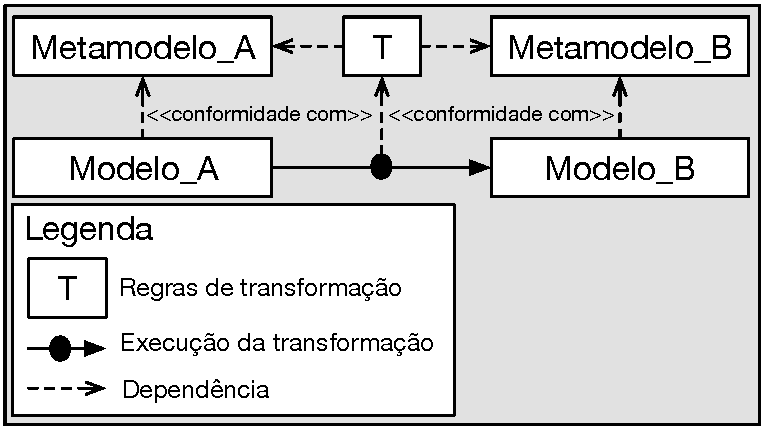
\includegraphics[scale=0.7]{images/transformacaoModeloA}
\label{fig:subfigure1}}
\quad
\subfigure[ \emph{endogenous} \aspas{\emph{in-place}}]{%
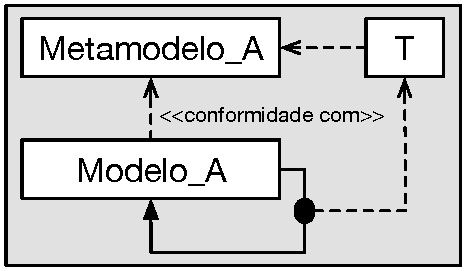
\includegraphics[scale=0.7]{images/transformacaoModeloB}
\label{fig:subfigure2}}
\label{fig:model_transformations}
 \fadaptada{Brambilla_2012}
\end{figure}

%\begin{figure}[htb]
% \caption{Diferentes tipos de transformações em modelos: (a) \emph{exogenous} \aspas{\emph{out-place}} vs. (b) \emph{endogenous} \aspas{\emph{in-place}}}
% \label{fig:model_transformations}
% \centering
% 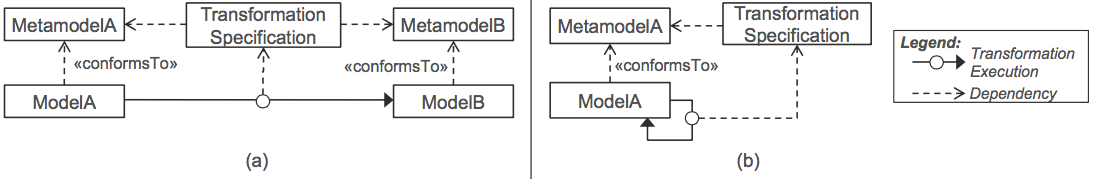
\includegraphics[scale=0.45]{images/transformacoes.png}
% \fadaptada{Brambilla_2012}
%\end{figure}

Transformações endógenas geralmente são implementadas utilizando técnicas de \aspas{reescrita de grafo}, ou como também é conhecida \aspas{transformação de grafo}~\cite{Ehrig_2006}. Na teoria dos grafos, \aspas{reescrita de grafo} é um conjunto de regras para reescrever um determinado grafo, por exemplo, dado $p: \emph{left-hand side} (LHS) \rightarrow \emph{right-hand side} (RHS)$, sendo $LHS$ o grafo usado como padrão (no lado esquerdo) e $RHS$ o grafo de substituição (no lado direito da regra). Mais precisamente, o lado esquerdo, LHS, representa todas pré-condições que devem ser satisfeitas antes da execução das regras de transformações. Similarmente, o lado direito, RHS, contém todas pós-condições. As ações que serão executadas pelas regras de transformações são implicitamente definidas tanto no grafo LHS, quanto no grafo RHS. A execução de um conjunto de regra de transformação produz os seguintes efeitos: (\textit{i}) todos elementos que apenas estão contidos no grafo LHS são deletados; (\textit{ii}) todos elementos que apenas estão contidos no grafo RHS são adicionados; (\textit{iii}) todos elementos que estão contidos em ambos os grafos, LHS e RHS, são preservados~\cite{Ehrig_2006}. 

Neste contexto, \aspas{reescrita de grafo} é útil para auxiliar na definição de transformações de modelos e metamodelos. Por exemplo, de acordo com~\citeonline{Lehnert_2012, Fluri_2006}, técnicas de \aspas{reescrita de grafo} podem ser aplicadas em qualquer metamodelo e modelos que implementam o padrão MOF, ou seja, KDM, UML, entre outros. Qualquer instância de um metamodelo que implemente o padrão MOF pode ser representada como um grafo da seguinte forma: (\textit{i}) vértices podem ser entendidos como: \texttt{EPackage}, \texttt{EClass}, \texttt{EDataType}, \texttt{EEnum}, \texttt{EAnotation}, \texttt{EOperation}, \texttt{EAttribute} e \texttt{EEnumLiteral}; (\textit{ii}) arestas podem ser representadas em metamodelo como: \texttt{EReference}, \texttt{Inheritance}, \texttt{EAnnotationLink}. Assim, pode-se definir e realizar evoluções, simulações, refatorações de modelos por meio de técnicas de \aspas{reescrita de grafo}. 

% Dessa forma, as gramáticas de um grafo consistem de um conjunto de regras de transformações e um grafo inicial (geralmente referenciado como grafo \aspas{hospedeiro}) onde as regras de transformações são aplicadas. Usualmente as regras de transformações consistem de um grafo denominado \emph{left-hand side} (LHS) e um grafo \emph{right-hand side} (RHS). O grafo LHS tem como intuito representar todas as pré-condições para antes do conjunto de regras de transformações serem aplicadas no modelos. Similarmente, o grafo RHS contêm todas as pós-condições. As ações que serão executadas pelas regras de transformações são implicitamente definidas tanto no grafo LHS quanto no grafo RHS. Mais precisamente, a execução de um conjunto de regra de transformação produz os seguintes efeitos: (\textit{i}) todos os elementos que apenas estão contidos no grafo LHS são deletados; (\textit{ii}) todos os elementos que apenas estão contidos no grafo RHS são adicionados; e (\textit{iii}) todos os elementos que estão contidos em ambos os grafos, LHS e RHS, são preservados. 

Comumente, transformações em modelos são desenvolvidas utilizando linguagens especializadas, denominadas de linguagens de transformação de modelos. Diversas linguagens de transformação de modelos têm sido propostas atualmente~\cite{Allilaire_06, Biehl_2010}. Cada linguagem tipicamente fornece um conjunto de características que a torna mais apropriada para o tipo de transformação almejada. No trabalho de~\citeonline{Biehl_2010}, são citadas várias linguagens de transformação de modelos, o que mostra uma dimensão do número de linguagens para transformação de modelos existentes e disponíveis para o usuário atualmente. Algumas das linguagens citadas são: ATL~\cite{ATL_eclipse,Jouault_2008}, \sigla{QVT}{\textit{Query/View/Transformation}}~\cite{QVT:OMG}, EMF Henshin~\cite{EMF_Henshin}, SmartQVT~\cite{SmartQVT}, ModelMorf~\cite{ModelMorf}, Kermeta~\cite{kermeta}, \sigla{ETL}{\textit{Epsilon Transformation Language}}~\cite{ETL_eclipse}, \sigla{OAW}{OpenArchitectureWare}~\cite{OpenArchitectureWare}, VIATRA~\cite{viatra}, AndroMDA~\cite{andromda} e Fujaba Transformations~\cite{fujaba}.

Nos trabalhos de~\citeonline{Biehl_2010, Mens_2006, Allilaire_06}, os autores buscam levantar características importantes tanto para classificar as transformações de modelos, quanto as linguagens de transformação de modelos  para realização dessas transformações. Similarmente,~\citeonline{transformation_huber} busca avaliar diferentes ferramentas e linguagens de transformação de modelos. O estudo conclui que nenhuma ferramenta é melhor do que a outra, mas que uma linguagem pode ser mais adequada para um problema específico do que outras linguagens. Entre as várias características utilizadas pelos autores na classificação das linguagens de transformação, a de maior importância é quanto ao paradigma da linguagem. Segundo~\citeonline{Mens_2006}, a maior distinção entre os mecanismos de transformação de modelos é quanto ao seu paradigma. Os principais paradigmas das linguagens de transformações de modelos são:

\begin{itemize}
	\item Imperativo: Linguagens imperativas especificam um fluxo de controle sequencial e fornecem meios para descrever a forma como a linguagem de transformação de modelo supostamente deve ser executada~\cite{Mens_2006}. As construções e conceitos de linguagens de transformações imperativas são semelhantes às linguagens de programação de propósito geral, como Java ou C;
	\item Declarativo: Linguagens declarativas não oferecem um fluxo de controle explícito. Em vez de se concentrar em como a transformação deve ser executada, o foco é sobre o que deve ser mapeado pela transformação~\cite{Mens_2006}. Transformações de modelos declarativas descrevem a relação entre os metamodelos fonte e alvo, e essa relação pode ser interpretada bidirecionalmente. Em geral, tais linguagens são compactas e as descrições de transformações são geralmente curtas e concisas~\cite{Biehl_2010, Mens_2006};
	\item Híbrido: Linguagens híbridas oferecem tanto as construções de linguagem imperativa, quanto as construções de linguagem declarativa;
	\item Transformação Direta: Linguagens de programação de uso geral e bibliotecas para ler e gravar os dados dos modelos são utilizadas para implementar as transformações de modelos~\cite{transformation_huber}. A vantagem da transformação direta é que os programadores não precisam aprender uma nova linguagem. Mas, por outro lado, as implementações tendem a se tornar maiores~\cite{Biehl_2010}.
\end{itemize}


%Na literatura é possível identificar um conjunto de linguagens especificadas para auxiliar a realização de transformações em modelos. Por exemplo, VIATRA [16], AGG [17], Henshin [18], ATOM [19], ETL, ATL, QVT. De acordo com Livro MDD ATL é a linguagem de transformações em modelos mais utilizada tanto academicamente quanto industrialmente. Dessa forma, nesta tese de doutorado optou-se por utilizar a ATL para a definição de transformações em modelos. Na subseção a seguir é apresentado como a ATL pode ser utilizada para a realização de transformações em modelos.

\subsection{ATLAS \emph{Transformation Language} (ATL)} % (fold)
\label{sub:atl_transformation_language}

A \sigla{ATL}{ATLAS \emph{Transformation Language}}~\cite{ATL_eclipse} é uma linguagem de transformação de modelo híbrida, ou seja, a linguagem contém uma mistura de construções declarativas e imperativas. O uso do estilo declarativo é encorajado por vários autores~\cite{Allilaire_06, Jouault_2005, Jouault_2008}, pois permite uma implementação mais objetiva e mais simples. No entanto, a definição de transformações complexas utilizando apenas construções declarativas pode ser uma tarefa difícil. Nesse caso, os desenvolvedores podem recorrer aos recursos imperativos da linguagem~\cite{Allilaire_06}.

A ATL possui uma sintaxe abstrata definida utilizando um metamodelo. Isso significa que cada transformação definida em ATL é de fato um modelo. Uma transformação ATL pode ser decomposta em três partes: um \textit{header}, \textit{helpers} e um conjunto de \textit{rules}. O \textit{header} (cabeçalho) é utilizado para declarar informações gerais, tais como o nome do módulo (nome da transformação que deve coincidir com o nome do arquivo .atl), os metamodelos de entrada e de saída  e a importação de bibliotecas necessárias. Os \textit{helpers} são sub-rotinas usadas para evitar a redundância de código. Pode-se imaginar um \textit{helper} como um método igual ao que se tem em linguagens de programação. Já as \textit{rules} (regras) são as principais definições das transformações ATL, porque elas descrevem como os elementos de saída (em conformidade com o metamodelo de saída) são produzidos a partir de elementos de entrada (em conformidade com o metamodelo de entrada). Elas são constituídas por ligações, cada uma expressando um mapeamento entre um elemento de entrada e um elemento de saída~\cite{ATL_eclipse}.

O funcionamento da ATL se dá da seguinte forma. Primeiro o código ATL deve ser compilado e, em seguida, executado pelo mecanismo de transformação ATL. A ATL oferece suporte dedicado para rastreabilidade e a ordem de execução das regras é determinada automaticamente, com exceção das \textit{Lazy Rules}, que precisam ser chamadas explicitamente no código da ATL. Os \textit{helpers} fornecem construções imperativas às transformações. A ATL também possui um módulo denominado ATL \textit{Refining} que suporta transformações do tipo \emph{endogenous} \aspas{\emph{in-place}} (ver Figura~\ref{fig:model_transformations}(b)).

A ATL foi escolhida para a implementação deste trabalho considerando vários aspectos. A ATL está integrada na plataforma Eclipse, o que provê uma série de recursos padrões para o desenvolvimento (\textit{syntax highlighting} e \textit{debugger}). A ATL é parte do projeto M2M da ferramenta Eclipse e possui um grupo de discussão ativo, constantemente atualizado. Vários exemplos e diversos estudos de casos aplicados até mesmo na indústria\footnote{\texttt{\texttt{https://www.eclipse.org/forums/index.php?t=thread&frm_id=241}}} utilizam a ATL e por se tratar de uma ferramenta de fácil uso, a partir de premissa de conhecimento de linguagem e do metamodelo, traz como vantagem ao processo: baixo custo, por ser uma ferramenta livre, e alta flexibilidade, por facilitar grandes alterações na transformação diretamente usando a interface do editor de regras ATL~\cite{Salem_2008}. Além disso, a ATL é uma das linguagens de transformações mais madura no contexto da MDE~\cite{bruneliere_2010}.
































%\subsection{Refatorações para Modelos}\label{sec:refactoringModel_section}


%Refatorações para modelos também têm-se a preocupação de preserva o comportamento após a aplicação de refatorações da mesma forma que refatorações tradicionais. A abordagem mais popular para definir a preservação de comportamento no contexto de modelos é por meio de restrições. Restrições são asserções que o modelo deve satisfazer antes e após a aplicação de refatoração. Tais asserções são representadas e definidas em nível de modelo por meio de pré- e pós-condições que devem ser validadas antes de executar a refatoração ou validados após a aplicação de refatorações. OCL é a linguagem mais utilizada na literatura para definir asserções para modelos.


\section{Modernização Dirigida a Arquitetura}\label{sec:modernizacaoOrientada_Arquitetura}


O crescente interesse na MDE motivou o \sigla{OMG}{\textit{Object Management Group}} a lançar a iniciativa denominada Modernização Dirigida a Arquitetura (do inglês - \textit{Architecture-Driven Modernization} (ADM)), cujo objetivo foi estabelecer metamodelos padronizados para auxiliar todo o  processo da reengenharia de software. Tal iniciativa foi motivada devido ao alto número de projetos de reengenharia de software que não obtiveram sucesso~\cite{Sneed_2005, Demeyer2}. Como resultado desse esforço, os conceitos da ADM foram criados, os quais possuem como objetivo revitalizar/modernizar softwares existentes\footnote{No contexto desse documento, softwares existentes e sistemas legados são utilizados de forma intercambiáveis} com a utilização de metamodelos padronizados, empregando os princípios da abordagem Arquitetura Dirigida a Modelo (do inglês - \sigla{MDA}{\textit{Model-Driven Architecture}}) (ver Seção~\ref{Cap2_Sec2_Desenvolvimento_Dirigido_a_Modelos}). %No contexto da ADM, todos os modelos são homogêneos, permitindo assim a criação de transformações \textit{Model-To-Model} M2M 

Entre os termos mais recentes relacionados à reengenharia de software, a ADM se destaca. De acordo com o OMG~\cite{OMG_OMG}, o objetivo da ADM não é substituir o processo tradicional da reengenharia de software, pelo contrário, a ADM almeja auxiliar e melhorar o processo de reengenharia de software por meio da utilização dos princípios da MDA. A ADM consiste em uma adaptação do modelo de ferradura tipicamente conhecido em reengenharia de software (i.e, o modelo de ferradura, basicamente contém dois lados, esquerdo, direito e uma \aspas{ponte} ligando os dois lados). Na Figura~\ref{fig:horse_shoe}, é apresentado o modelo de ferradura adaptado para a ADM e é importante observar que essa figura contém todas as fases e \aspas{palavras-chaves} tradicionais que são encontradas na reengenharia de software tradicional e em MDA, tais como: Modelo Específico de Plataforma (do inglês - \textit{Platform-Specific Model} (PSM)), Modelo Independente de Plataforma (do inglês - \textit{Platform-Independent Model} (PIM)) e Modelo Computacional Independente (do inglês - \textit{Computation-Independent Model} (CIM)). As fases tradicionais da reengenharia de software adaptadas para a ADM são:


\begin{itemize}
 	\item \textbf{Engenharia Reversa}: essa fase tem como entrada um sistema que será modernizado, e, posteriormente, esse sistema será transformado em um PSM. Além disso, o PSM é utilizado como entrada para a geração do PIM, que, no contexto dessa tese, consiste em uma instância do metamodelo denominado KDM (ver Seção~\ref{sec:knowledge_discovery_meta_model});
 	\item \textbf{Reestruturação}: nessa fase, um conjunto de reestruturação/refatoração pode ser aplicado sobre uma instância do metamodelo KDM por meio de transformações de modelo para modelo (do inglês - \sigla{M2M}{\emph{Model-To-Model}});
 	\item \textbf{Engenharia Avante}: nesta fase um novo código-fonte do sistema modernizado é gerado automaticamente por meio de transformações de modelo para código (do inglês - \sigla{M2C}{\emph{Model-To-Code}}). 
 \end{itemize} 

 \begin{figure}[htb]
 \caption{Modelo de ferradura adaptada para a ADM.}
 \label{fig:horse_shoe}
 \centering
 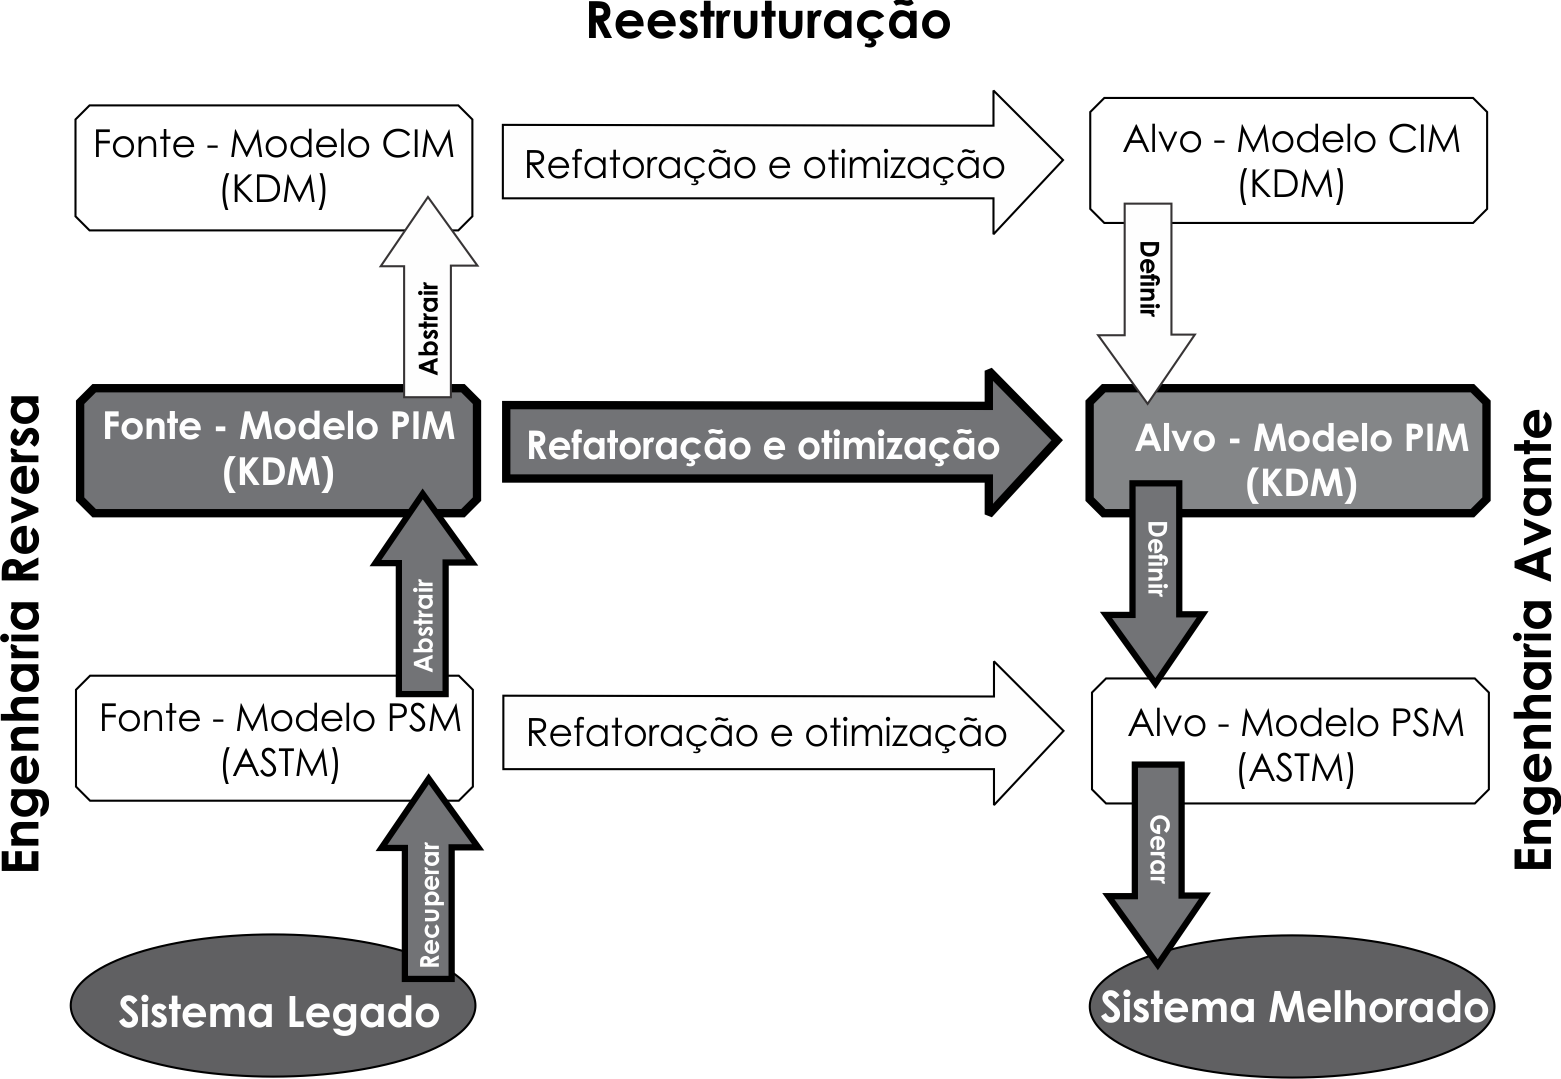
\includegraphics[scale=0.78]{images/modelo-ferradura.png}
 \fadaptada{ADM:OMG}
\end{figure}

Durante o processo da ADM, todos os modelos (i.e., PSM, PIM e CIM) podem estabelecer transformações/refatorações entre si, como ilustrado na Figura~\ref{fig:horse_shoe}. Geralmente, tais transformações são executadas por meio de linguagens de transformações. Como salientado no Capítulo~\ref{chapter:fundamentacao_teorica}, Seção~\ref{sec:transformacoes_de_modelos}, usualmente essas transformações são implementadas utilizando diferentes linguagens de transformações, que podem ser declarativas, imperativas ou híbridas. 

É importante também destacar que a ADM não tem como intuito apenas seguir todos os princípios da abordagem MDA~\cite{ADM:OMG}. Um dos principais objetivos da ADM é definir um conjunto de metamodelos padronizados para lidar com diferentes desafios que são encontrados hoje em dia na reengenharia de software. Dessa forma, em Novembro de 2003, a \sigla{ADMTF}{\textit{Architecture-Driven Modernization Task Force}} criou uma \sigla{RFP}{\textit{Request-for-Proposal}}, que, por sua vez descrevia um conjunto de metamodelos. Tais metamodelos são: (\textit{i}) Knowledge Discovery Metamodel (KDM), maiores informações sobre esse metamodelo são apresentadas na seção~\ref{sec:knowledge_discovery_meta_model}, (\textit{ii}) \sigla{SMM}{\textit{Structured Metrics metamodel}}, que é um metamodelo para representar e definir métricas e resultados de medições, (\textit{iii}) \sigla{ADMPR}{\textit{ADM Pattern Recognition}}, que facilita a busca de padrões em um software, (\textit{iv}) \sigla{ADMVS}{\textit{ADM Visualization Specification}}, que tem como objetivo representar visualmente metadados de uma aplicação representada em KDM, (\textit{v}) \sigla{ADMRS}{\textit{ADM Refactoring Specification}}, que almeja definir um metamodelo padronizado para especificar e definir refatorações, utilizando outros metamodelos da ADM, como por exemplo o KDM. O estado atual de cada metamodelo pode ser visto na Tabela~\ref{tab:todos_os_meta_modelos_da_ADM}~\cite{ADM:OMG}, a qual mostra que alguns metamodelos ainda encontram-se em fase de desenvolvimento e outros já foram finalizadas e disponíveis pelo OMG.

% Please add the following required packages to your document preamble:
% \usepackage{multirow}
\begin{table}[h]
\centering
\caption{Estado atual dos metamodelos da ADM.}
\label{tab:todos_os_meta_modelos_da_ADM}
\begin{tabular}{|l|l|l|l|}
\hline
\multicolumn{1}{|c|}{Metamodelo}                                         & \multicolumn{1}{c|}{Situação}           & \multicolumn{1}{c|}{Versão} & \multicolumn{1}{c|}{Data}          \\ \hline
\textit{ADM Pattern Recognition} (ADMPR)                     & Em desenvolvimento &\multicolumn{1}{c|}{\textemdash}&\multicolumn{1}{c|}{\textemdash}\\ \hline
\textit{ADM Refactoring Specification} (ADMRS)               & Em desenvolvimento &\multicolumn{1}{c|}{\textemdash}&\multicolumn{1}{c|}{\textemdash}\\ \hline
\textit{ADM Visualization Specification} (ADMVS)             & Em desenvolvimento &\multicolumn{1}{c|}{\textemdash}&\multicolumn{1}{c|}{\textemdash}\\ \hline
\sigla{ASTM}{\textit{Abstract Syntax Tree Metamodel}}               & \multicolumn{1}{c|}{Disponível}         & \multicolumn{1}{c|}{1.0}    & \multicolumn{1}{c|}{2011}  \\ \hline
\textit{Knowledge Discovery Metamodel} (KDM)                 & \multicolumn{1}{c|}{Disponível}         & \multicolumn{1}{c|}{1.3}    & \multicolumn{1}{c|}{2011}   \\ \hline
\multirow{2}{*}{\textit{Structured Metrics Metamodel} (SMM)} & \multicolumn{1}{c|}{Disponível}         & \multicolumn{1}{c|}{1.0}    & \multicolumn{1}{c|}{2012}  \\ \cline{2-4} 
                                                    & Em desenvolvimento & \multicolumn{1}{c|}{1.1}    & \multicolumn{1}{c|}{2013} \\ \hline
\end{tabular}
\end{table}

É importante destacar que a abordagem proposta nesta tese se concentra no metamodelo KDM. Consequentemente, é de suma importância o entendimento desse metamodelo, por isso, ele é mais detalhado neste capítulo.
KDM é um metamodelo que pode ser utilizado para representar todos os artefatos de um determinado software existente, por exemplo, nele há metaclasses específicas para representar desde código-fonte até a arquitetura de um determinado software. O KDM é um metamodelo de representação intermediária comum para sistemas existentes e seus ambientes operacionais. Utilizando esse metamodelo para sistemas existentes, é possível trocar representações do sistema em modelo entre plataformas e linguagens com a finalidade de analisar, padronizar e transformar/refatorar os sistemas existentes~\cite{ADM:OMG}. 

A ideia por trás do KDM é que a comunidade comece a criar analisadores sintáticos (do inglês - \textit{parsers}) para diferentes linguagens de programação, que transformem os códigos-fontes em instâncias do metamodelo KDM. Como resultado, qualquer técnica, ferramenta e abordagem que utilize o KDM como o artefato de entrada pode ser considerada uma técnica, ferramenta e/ou abordagem independente de linguagem e de plataforma. Por exemplo, um catálogo de refatoração para o KDM~\cite{durelli_catalogo, durelli_VEM_ferramenta} pode ser usado para refatorar vários sistemas independentemente da linguagem de programação. Maiores informações sobre o KDM, bem como sobre seus pacotes, metaclasses e metarrelacionamentos são apresentados a seguir.

\section{Knowledge Discovery Metamodel (KDM)}
\label{sec:knowledge_discovery_meta_model}

\sigla{KDM}{Knowledge Discovery Metamodel} é um metamodelo que representa existentes artefatos de software, seus elementos, associações e ambientes operacionais. O KDM tem como principal objetivo permitir que os engenheiros de modernização criem ferramentas para auxiliar a modernização de software, as quais sejam independentes de plataforma e linguagem~\cite{KDM:specification, PerezCastillo:2011jo, ADMCHAPTERR}. Além disso, o KDM facilita e assegura a interoperabilidade e a troca de dados entre diferentes ferramentas. 

Um problema tradicional facilmente identificado em várias ferramentas que lidam com a reengenharia de software é que tais ferramentas analisam diversos artefatos de um determinado software (por exemplo, código-fonte, banco de dados, \textit{scripts}, etc.) para obter conhecimentos explícitos, com o intuito de realizar transformações/refatorações~\cite{rosenberg, Canfora2011}. Como consequência, cada ferramenta gera e analisa tais conhecimentos de forma implícita. Assim, os conhecimentos gerados são restritos a uma específica linguagem de programação, e/ou a uma plataforma. Como resultado, tais restrições podem criar dificuldades com relação à interoperabilidade entre diferentes ferramentas. O KDM fornece uma estrutura que busca facilitar a troca de dados entre diversas ferramentas. Além disso, possui um conjunto de metaclasse e uma estrutura padronizada que fornecem meios para especificar desde artefatos físicos até artefatos lógicos de um determinado sistema de software. Em virtude dessa padronização, todas as técnicas/abordagem/ferramentas que utilizam o KDM como entrada podem ser consideradas independentes de plataforma e linguagem, aumentando, assim, a interoperabilidade e o reúso. Em 2012, o KDM tornou-se \sigla{ISO}{\emph{International Standards Organization}}~\cite{KDM:ISO} como uma estrutura que facilita a troca de dados entre as diversas ferramentas. O KDM é definido via \sigla{MOF}{\emph{Meta-Object Facility}}~\cite{MOF} e estabelece o formato de troca de dados via \sigla{XMI}{\emph{XML Metadata Interchange}}, o qual é denominado KDM XMI \emph{schema}.

Resumidamente, as principais metas do KDM são~\cite{ADM:OMG}: (\textit{i}) representa artefatos de um sistema legado como entidades, relacionamentos e atributos; (\textit{ii}) suporta uma variedade de plataformas e linguagens; (\textit{iii}) define uma terminologia unificada para artefatos de sistemas legados; (\textit{iv}) representa estruturas lógicas e físicas de sistemas legados; (\textit{v}) permite a modificação/refatoração de sistemas legados utilizando os princípios da MDA; (\textit{vi}) facilita o rastreamento de mudança entre artefatos; (\textit{vii}) facilita a sincronização de estruturas lógicas e físicas de um determinado sistema legado; (\textit{viii}) contém metaclasses para representar desde código-fonte até metaclasses para representar elementos arquiteturais de um determinado sistema legado.

%\begin{itemize}
	%\item KDM representa artefatos de um sistema legado como entidades, relacionamentos e atributos;
	%\item KDM suporta uma  variedade de plataforma e linguagem;
%	\item KDM define uma terminologia unificada para artefatos de sistemas legados;
	%\item KDM representa estruturas lógicas e físicas de sistemas legados;
	%\item KDM permite a modificação/refatoração de sistemas legados utilizando os princípios da MDA;
	%\item KDM facilita o rastreamento de mudança entre artefatos;
	%\item KDM facilita a sincronização de estruturas lógicas e físicas de um determinado sistema legado;
	%\item KDM contém metaclasses para representar desde código-fonte até metaclasses para representar elementos arquiteturais de um determinado sistema legado.
%\end{itemize}

De acordo com~\citeonline{PerezCastillo:2011jo}, o KDM busca cobrir um amplo escopo para abranger um conjunto diversificado de aplicações, plataformas e linguagens de programação, além de almejar fornecer a capacidade de troca de metadados entre diversas ferramentas e, assim, facilitar a cooperação entre fornecedores para integrar e aumentar a interoperabilidade de diferentes abordagens, técnicas, algoritmos, etc. A fim de alcançar essa interoperabilidade e, especialmente, a integração de informações sobre diferentes facetas de um determinado sistema a partir de múltiplas ferramentas, o KDM define vários níveis de conformidade, aumentando a probabilidade de que duas ou mais ferramentas apoiaram o mesmo metamodelo. Além disso, o KDM também é estruturado de forma modular, seguindo o princípio da separação de interesse, com a capacidade de representar partes heterogêneas de um sistema. A separação de interesses no contexto do metamodelo KDM é alcançada por meio de pacotes, como apresentado na Figura~\ref{kdm:domain}. Cada pacote está em um nível de conformidade e visa definir um ponto de vista arquitetural do sistema. Em outras palavras, cada pacote do KDM constitui uma determinada ontologia para descrever e representar a grande maioria dos artefatos de sistemas de software existentes. Por exemplo, os pacotes \texttt{Code} e \texttt{Action} contêm metaclasses que representam o código-fonte de um sistema, tais como, variáveis, procedimentos/métodos/funções, chamadas para métodos, etc. Similarmente, o pacote \texttt{Structure} contém metaclasses para representar elementos arquiteturais do sistema, tais como, componentes, camadas, subcomponentes, etc. O pacote \texttt{Conceptual} possui  metaclasses para definir regras de negócio do sistema.


\begin{figure}[htb]
 \caption{Pacotes e nível de conformidade do metamodelo KDM.}
 \label{kdm:domain}
 \centering
 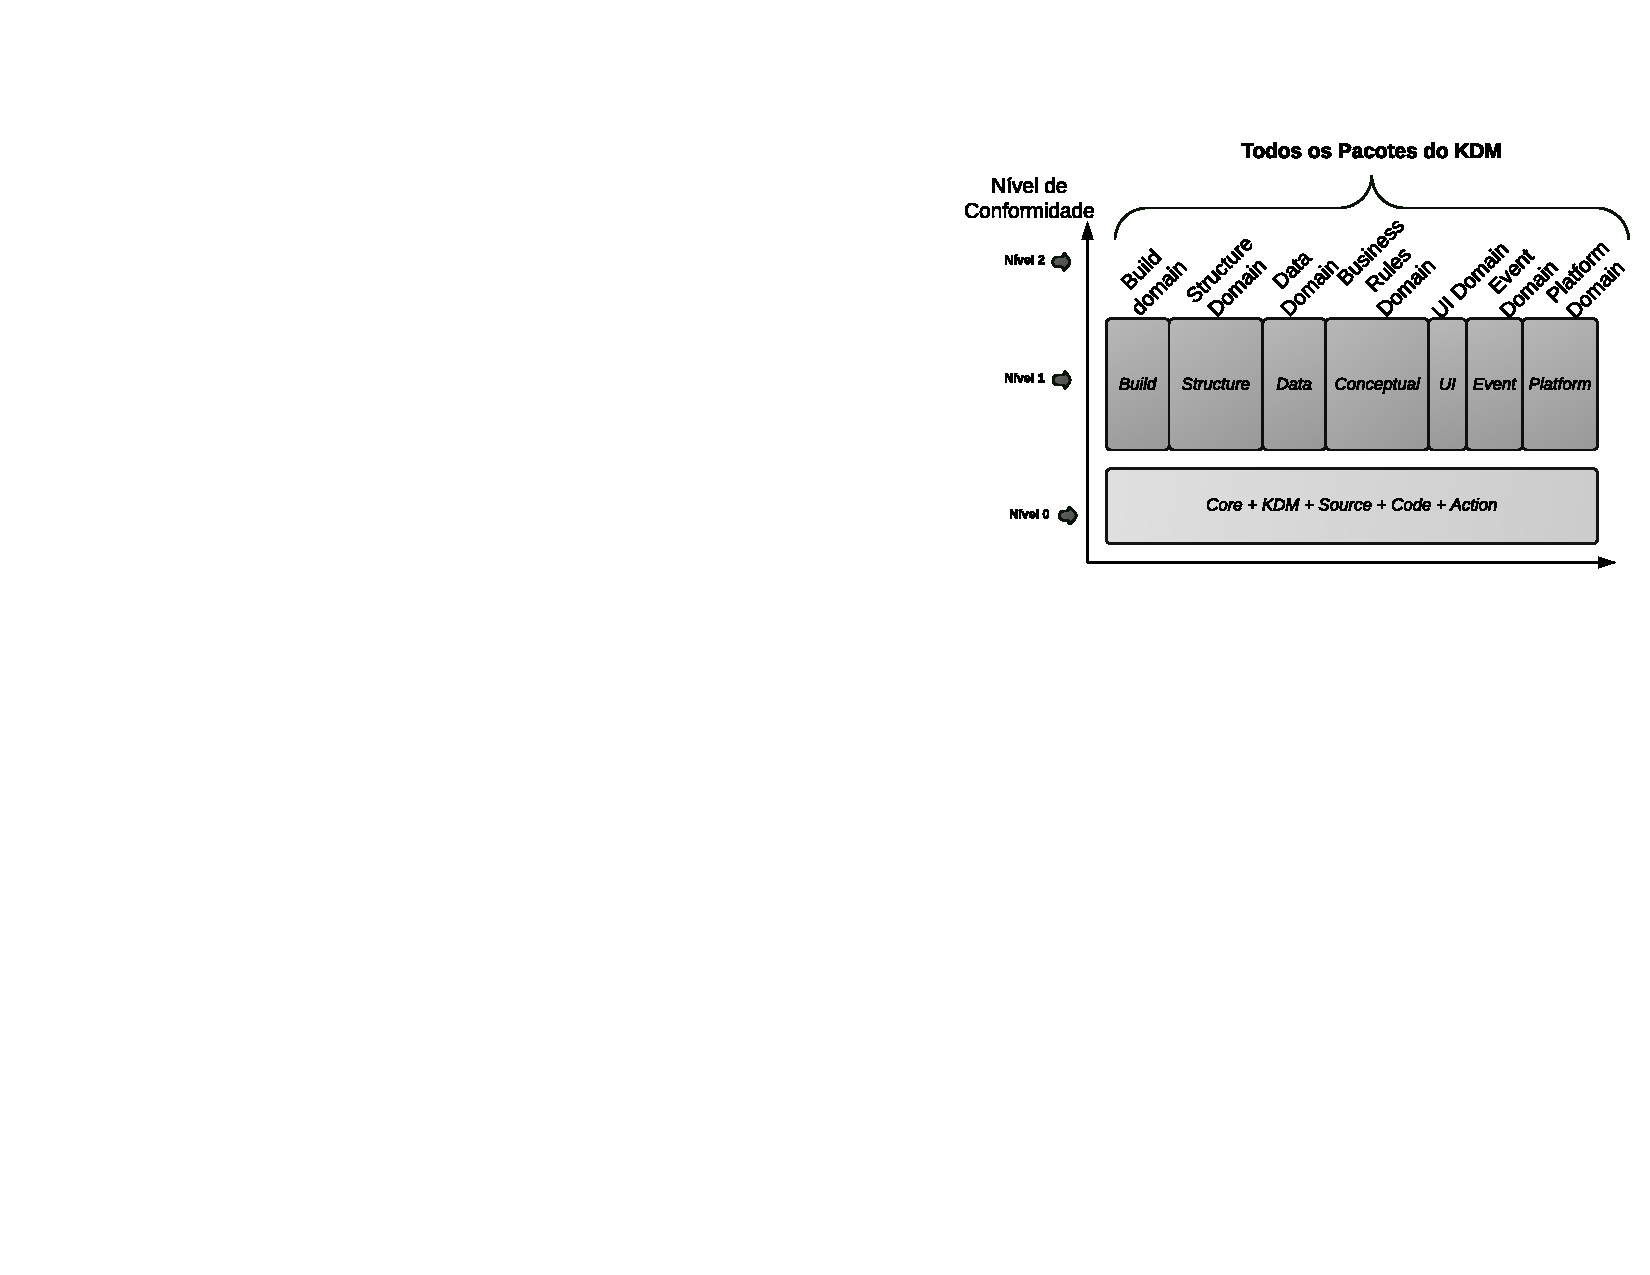
\includegraphics[scale=1]{images/kdmLevels_pacotes.pdf}
 \fadaptada{KDM:specification}
\end{figure}

Da perspectiva de um engenheiro de modernização, essa separação de interesse do KDM, por meio de pacote, significa que o engenheiro só precisa se preocupar com os pacotes do KDM que considerar necessários para as suas atividades de modernização, por exemplo, uma determinada abordagem pode necessitar apenas do pacote \texttt{Code} e \texttt{Action}, enquanto outra abordagem pode utilizar apenas o pacote responsável por definir elementos arquiteturais. Se essas abordagens forem evoluídas ao longo do tempo e necessitarem de outros pacotes do KDM, pacotes podem ser adicionados ao repertório da abordagem/ferramenta, conforme necessário.

Como observado na Figura~\ref{kdm:domain}, o KDM possui três níveis de conformidade, nível 0, nível 1 e nível 2. Cada nível é apresentado a seguir:

\begin{itemize}
    \item \textbf{Nível 0}: nesse nível, são definidos os seguintes pacotes do KDM: (\textit{i})     \texttt{Core}, (\textit{ii}) \texttt{kdm}, (\textit{iii}) \texttt{Source}, (\textit{iv}) \texttt{Code} e (\textit{v}) \texttt{Action}. Esse nível de conformidade representa um denominador comum que pode servir como uma base para a interoperabilidade entre diferentes categorias de ferramentas que utilizem o metamodelo KDM. Para que uma ferramenta esteja em conformidade com o \textbf{Nível 0}, ela deve fornecer completo suporte para todas as metaclasses que foram definidas nos pacotes \texttt{Core}, \texttt{kdm}, \texttt{Source}, \texttt{Code} e \texttt{Action};
    \item \textbf{Nível 1}: nesse nível, os pacotes definidos no \textbf{Nível 0} são estendidos para representar outros artefatos de um determinado sistema. Além disso, o \textbf{Nível 1} define os seguintes pacotes: (\textit{i}) \texttt{Build}, (\textit{ii}) \texttt{Structure}, (\textit{iii}) \texttt{Data}, (\textit{iv}) \texttt{Conceptual}, (\textit{v}) \texttt{UI}, (\textit{vi}) \texttt{Event} e (\textit{vii}) \texttt{Platform}. Para que uma ferramenta esteja em conformidade com o \textbf{Nível 1} ela deve fornecer suporte para todos os pacotes do \textbf{Nível 0} pelo menos um dos pacotes do \textbf{Nível 1};
    \item \textbf{Nível 2}: esse nível é a união de todos os pacotes definidos no nível anterior. Para que uma ferramenta esteja em conformidade com o \textbf{Nível 2}, ela deve fornecer suporte para todos os pacotes do \textbf{Nível 1} e pelo menos um do \textbf{Nível 2}.
\end{itemize}


Todos os pacotes do metamodelo KDM apresentados na Figura~\ref{kdm:domain} são organizados em quatro camadas de abstração: (\textit{i}) \sigla{CI}{Camada de Infraestrutura}: do inglês \textit{Infrastructure Layer}; (\textit{ii}) \sigla{CEP}{Camada de Elementos de Programa}: do inglês \textit{Program Elements Layer}; (\textit{iii}) \sigla{CRTE}{Camada de Recurso de Tempo de Execução}: do inglês \textit{Runtime Resource Layer}; (\textit{iv}) \sigla{CA}{Camada de Abstração}: do inglês \textit{Abstraction Layer}. Essas quatro camadas estão apresentadas esquematicamente na Figura~\ref{fig:kdm_layer}.

%\begin{itemize}
    %\item \sigla{CI}{Camada de Infraestrutura}: do inglês \textit{Infrastructure Layer};
    %\item \sigla{CEP}{Camada de Elementos de Programa}: do inglês \textit{Program Elements Layer};
    %\item \sigla{CRTE}{Camada de Recurso de Tempo de Execução}: do inglês \textit{Runtime Resource Layer};
    %\item \sigla{CA}{Camada de Abstração}: do inglês \textit{Abstraction Layer}.
%\end{itemize}


%(\textit{i}) \sigla{CI}{Camada de Infraestrutura} (do inglês \textit{Infrastructure Layer}), (\textit{ii}) \sigla{CEP}{Camada de Elementos de Programa} (do inglês \textit{Program Elements Layer}), (\textit{iii}) \sigla{CRTE}{Camada de Recurso de Tempo de Execução} (do inglês \textit{Runtime Resource Layer}) e (\textit{iv} ) \sigla{CA}{Camada de Abstração} (do inglês \textit{Abstraction Layer}). 

%Cada camada é posteriormente organizada em pacotes, como pode ser observado na Figura~\ref{fig:kdm_layer}. Por sua vez, cada pacote define um conjunto de metaclasses cujo propósito é representar o conhecimento de específicos artefatos de um determinado sistema. 

%
\begin{figure}[htb]
 \caption{Camadas e pacotes do KDM.}
 \label{fig:kdm_layer}
 \centering
 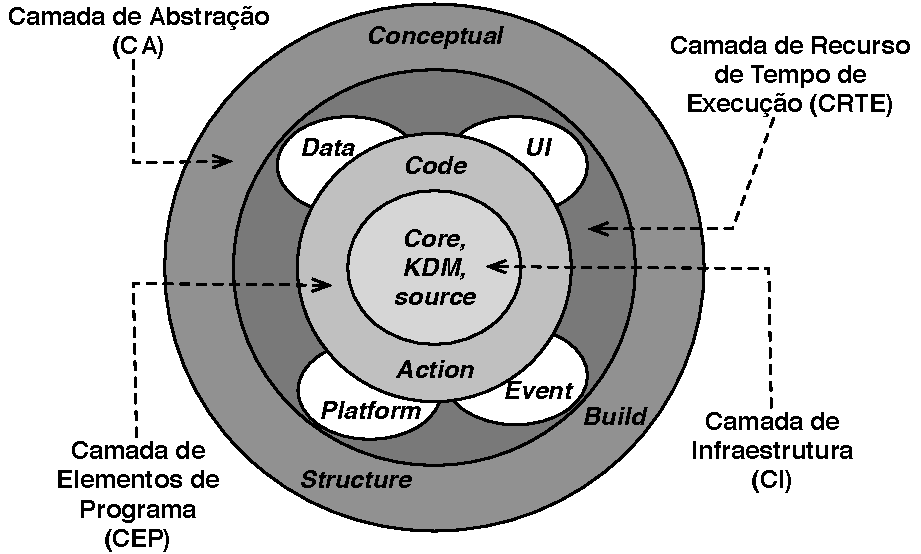
\includegraphics[scale=0.67]{images/kdm_layers.pdf}
 \fadaptada{KDM:specification}
\end{figure}
%
A camada CI contém três pacotes, e são eles: (\textit{i}) \texttt{Core}, (\textit{ii}) \texttt{\aspas{kdm}} e (\textit{iii}) \texttt{Source}. Os dois primeiros pacotes, \texttt{Core} e \texttt{\aspas{kdm}}, representam a infraestrutura básica para outros pacotes do KDM e definem metaclasses e relacionamentos básicos. O pacote \texttt{Source} define o \texttt{Inventory Model}, o qual representa artefatos de software e mantém a rastreabilidade entre eles. 

A camada CEP possui dois pacotes: (\textit{i}) \texttt{Code} e (\textit{ii}) \texttt{Action}, os quais coletivamente definem o \texttt{Code Model} que contém metaclasses para representar artefatos no âmbito da implementação. O pacote \texttt{Code} apresenta um conjunto de metaclasses para representar a estrutura de um determinado programa e seus relacionamentos, já o pacote \texttt{Action} possui metaclasses para descrever o comportamento e o fluxo de dados de um programa.

A camada CRTE compreende quatro pacotes: (\textit{i}) \texttt{Data}, (\textit{ii}) \texttt{Platform}, (\textit{iii}) \texttt{Event} e (\textit{iv}) \texttt{UI}. Coletivamente, tais pacotes representam a estrutura e o comportamento de recursos de tempo de execução do sistema. Tais pacotes são diretamente instanciados por meio da definição de recursos, abstração do \texttt{Code Model}, ou, ainda, são manualmente instanciados pelo engenheiro de modernização. A rastreabilidade entre os elementos abstraídos e os elementos físicos (por exemplo, código-fonte) é mantida pelo meta-atributo, denominado \texttt{implementation}. Finalmente, a camada CA engloba três pacotes: (\textit{i}) \texttt{Conceptual}, (\textit{ii}) \texttt{Structure} e (\textit{iii}) \texttt{Build} possuindo metaclasses para representar o maior nível de abstração de um sistema, por exemplo, a estrutura do sistema, regras de negócios, documentações do sistema, etc.

Uma característica importante de ser observada e ressaltada é que todas as camadas do KDM interagem, significando que todas elas são conectadas de alguma forma\footnote{Essas conectividades entre os elementos de cada camada são mantidas por um conjunto de meta-atributo, por exemplo, o meta-atributo \textit{implementation}.}, e, como consequência, se uma mudança/refatoração for realizada em uma camada específica, a mudança/refatoração deverá ser propagada para outras camadas com o intuito de manter todas as camadas sincronizadas e consistentes preservando, assim, a estrutura sintática e semântica do KDM. Nas próximas seções, são apresentados os principais pacotes do metamodelo KDM que compõem o contexto para o desenvolvimento deste trabalho.

\subsection{Pacote Code}\label{subsection:codePackage}

O pacote $\mathtt{Code}$ define um conjunto de metaclasses, cujo propósito é representar unidades de programa em nível de implementação e às suas associações. O pacote também inclui metaclasses que representam elementos de programa comuns e suportados por várias linguagens de programação, como: tipos de dados, classes, procedimentos, macros, protótipos e \textit{templates}.


Em uma determinada instância do KDM, cada elemento do pacote~$\mathtt{code}$ representa alguma construção em uma linguagem de programação, determinada pela linguagem de programação utilizada no sistema. Na Figura~\ref{fig:CodeModel}, um trecho do~$\mathtt{CodeModel}$\footnote{O diagrama de classes do $\mathtt{CodeModel}$, mostrado aqui, só representa o conjunto de metaclasses e os seus respectivos relacionamentos lógicos (para informações completas, verifique a especificação do KDM~\cite{KDM:specification}.} é retratado.

%In a given KDM instance, each instance of the code metamodel element represents some programming language construct, determined by the programming language of the existing software system. Each instance of a code metamodel element corresponds to a certain region of the source code in one of the artifacts of the existing software system. Figure~\ref{fig:CodeModel} the \texttt{CodeModel}\footnote{The \texttt{CodeModel} class diagram presented herein shows just a set of the metaclasses and their logical relationship, for complete information please see the KDM specification} is depicted, it represents parts of the KDM infrastructure. 

\begin{figure}[!ht]
	\centering
	% Requires \usepackage{graphicx}
	\caption{Diagrama de classes - $\mathtt{CodeModel}$}
	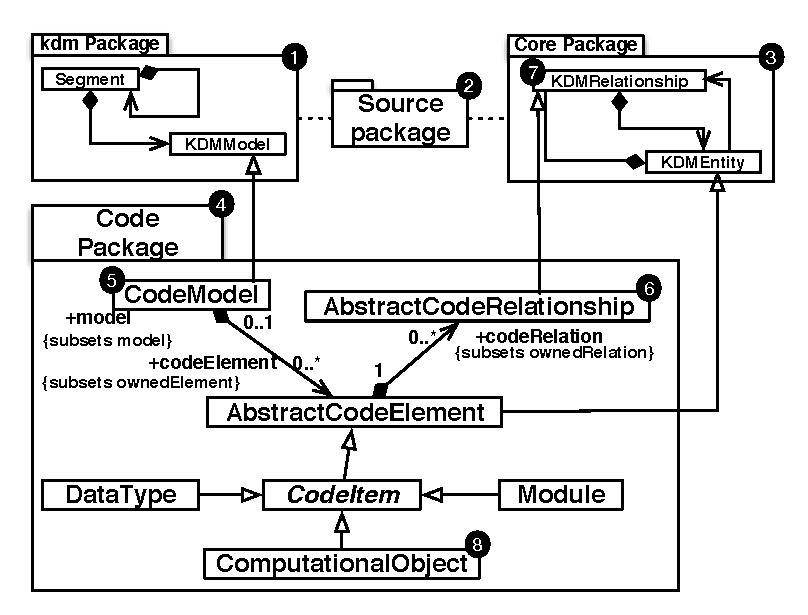
\includegraphics[scale=0.67]{images/codeModel}
	\label{fig:CodeModel}
	\fadaptada{KDM:specification}
\end{figure}

A metaclasse \texttt{CodeModel} representa um contêiner para outras instâncias de elementos do tipo~$\mathtt{Code}$. O pacote $\mathtt{Code}$ \ding{205} depende dos outros pacotes $\mathtt{kdm}$ \ding{202}, $\mathtt{Source}$ \ding{203} e $\mathtt{Core}$ \ding{204}. A metaclasse $\mathtt{CodeModel}$ \ding{206} é um modelo que possui coleções de fatos sobre o sistema de software, correspondentes ao domínio $\mathtt{Code}$ e ela possui uma associação \texttt{codeElement:AbstractCode\-Ele\-ment[0..*]}, permitindo a adição de novos elementos de código, por exemplo, métodos, atributos, etc. A metaclasse  $\mathtt{AbstractCodeRelationship}$ \ding{207} representa qualquer relacionamento determinado por uma linguagem de programação. Por sua vez, a metaclasse $\mathtt{ComputationalObject}$ representa os elementos determinados pela linguagem de programação, que descreve certos objetos computacionais em tempo de execução, por exemplo, métodos e variáveis.

%This metamodel element is a container for other \texttt{code} element instances. As can be observed in Figure~\ref{fig:CodeModel} the \texttt{Code} package \ding{205} depends on the \texttt{kdm} \ding{202}, \texttt{Source} \ding{203}, and \texttt{Core} \ding{204} packages. The meta-class \texttt{CodeModel} \ding{206} is the specific KDM model that owns collections of facts about the existing software system such that these facts correspond to the \texttt{Code} domain, its superclass is \texttt{KDMModel}. It has as association \texttt{codeElement:AbstractCodeElement[0..*]} meaning that one shall arrange code elements (e.g., methods, fields, etc) into one or more code models. The \texttt{AbstractCodeRelationship} \ding{207} is an abstract meta-class representing any relationship determined by a programming language, it is also used to constrain the subclasses of \texttt{KDMRelationship} (see Figure~\ref{fig:CodeModel} \ding{208}) in the \texttt{Code} model. The meta-class \texttt{ComputationalObject} represents the named elements determined by the programming language, which describe certain computational objects at the runtime, for example, methods, and variables.

O pacote~$\mathtt{Code}$ compreende em um total de 24 metaclasses, que são um arranjo de abstrações para representar toda a estrutura estática (ou grande maioria) de um terminado código-fonte, dada uma linguagem de programação, seja ela procedural ou orientada a objetos~\cite{KDM:specification}. Na Tabela~\ref{tab:meta_classes_pacoteCODE}, algumas metaclasses são apresentadas. É visto que algumas metaclasses podem ser diretamente elucidadas e mapeadas, como por exemplo, \aspas{classes} e \aspas{interfaces} construções facilmente encontradas em linguagens orientadas a objetos podem ser facilmente mapeada para as metaclasses denominada $\mathtt{ClassUnit}$ e $\mathtt{InterfaceUnit}$, respectivamente. Um mapeamento mais completo entre elementos estruturais e metaclasses do KDM pode ser identificado em~\citeonline{bruno_marinho_dissertacao} e no Capítulo~\ref{chapter:catalogo_refactoring_KDM}. Uma representação dessas metaclasses, bem como seus relacionamentos são apresentados em diagrama de classe na Figura~\ref{fig:classUnit_e_InterfaceUnit}.

\begin{figure}[!ht]
	\centering
	\caption{Diagrama de classes elucidando as metaclasses \texttt{ClassUnit} e \texttt{InterfaceUnit}}
	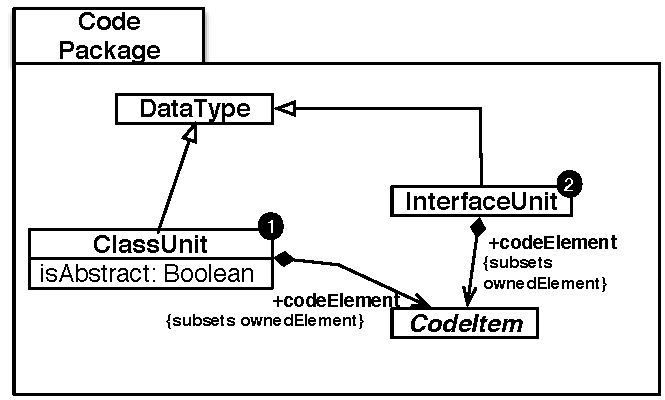
\includegraphics[scale=0.67]{images/ClassUnit_InterfaceUnit}
	\label{fig:classUnit_e_InterfaceUnit}
	\fadaptada{KDM:specification}
\end{figure}

%The whole \texttt{Code} package consists of $24$ metaclasses\footnote{Note that not all the meta-class are shown in Figure~\ref{fig:CodeModel}} and contains all the abstract elements for modeling the static structure of the source code. In Table~\ref{tab:mappingCodeToKDM} is depicted some of them. This table identifies KDM metaclasses possessing similar characteristics to the static structure of the source code. Some metaclasses can be direct mapped, such as class from object-oriented language, which can be easily mapped to the \texttt{ClassUnit} meta-class from KDM. For instance, the meta-class \texttt{Package} is a subtype for \texttt{Module} that logical collections of program elements, as directly supported by some programming languages, such as Java. 

\begin{table}[h]
\centering
\caption{Metaclasses para modelagem de estruturas estáticas do código-fonte.}
\label{tab:meta_classes_pacoteCODE}
\begin{tabular}{|l|l|}
\hline
Elemento do Código-Fonte & metaclasses do KDM \\ \hline
\multicolumn{1}{|c|}{Classe}                   & \multicolumn{1}{|c|}{\texttt{ClassUnit}}           \\ \hline
\multicolumn{1}{|c|}{Interface}                & \multicolumn{1}{|c|}{\texttt{InterfaceUnit}}       \\ \hline
\multicolumn{1}{|c|}{Método}                   & \multicolumn{1}{|c|}{\texttt{MethodUnit}}          \\ \hline
\multicolumn{1}{|c|}{Atributo}                 & \multicolumn{1}{|c|}{\texttt{StorableUnit}}        \\ \hline
\multicolumn{1}{|c|}{Variável Local}           & \multicolumn{1}{|c|}{\texttt{MemberUnit}}          \\ \hline
\multicolumn{1}{|c|}{Parâmetro}                & \multicolumn{1}{|c|}{\texttt{ParameterUnit}}       \\ \hline
\multicolumn{1}{|c|}{Associação}               & \multicolumn{1}{|c|}{\texttt{KDMRelationShip}}     \\ \hline
\end{tabular}
\end{table}

%\begin{table}[!h]
	%\caption{metaclasses para modelagem de estruturas estáticas do código fonte}
%	\label{tab:mappingCodeToKDM}
%	\centering
%	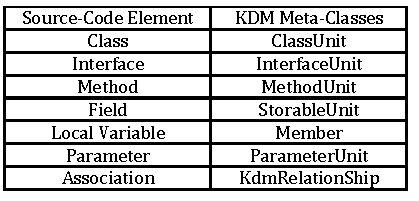
\includegraphics[scale=1]{images/tabela_comparativo_KDM_code_com_source_code}
%\end{table}

$\mathtt{ClassUnit}$ e $\mathtt{InterfaceUnit}$ representam \aspas{classes} e \aspas{interfaces} que são definidas por usuários de linguagens orientadas a objeto. Essas metaclasses possuem características e relacionamentos similares, como observado na Figura~\ref{fig:classUnit_e_InterfaceUnit} \ding{202} e \ding{203}. Uma das diferenças que pode ser destacada é que a metaclasse ~$\mathtt{ClassUnit}$ contém um meta-atributo~$\mathtt{isAbstract:Boolean}$, o qual é utilizado para especificar se uma classe é ou não abstrata. $\mathtt{ClassUnit}$ e $\mathtt{InterfaceUnit}$ podem conter uma coleção de elementos que seja do tipo ~$\mathtt{CodeItem}$, por exemplo,~$\mathtt{StorableUnit}$ ou ~$\mathtt{MethodUnit}$. Além disso, tais metaclasses  possuem uma meta-associação denominada ~$\mathtt{codeElement:CodeItem[0..*]}$, que é utilizada para agrupar todos membros da classe, por exemplo, construtores, métodos, atributos, etc. Na Figura~\ref{fig:StorableUnit_MethodUnit}, são apresentados os meta-atributos e of metarrelacionamentos das metaclasses \texttt{StorableUnit} \ding{204}, \texttt{MethodUnit} \ding{205}, \texttt{ParameterUnit} \ding{207} e \texttt{MemberUnit} \ding{206}.

\begin{figure}[!ht]
	\centering
	% Requires \usepackage{graphicx}
	\caption{Diagrama de classes elucidando as metaclasses \texttt{StorableUnit}, \texttt{MethodUnit}, \texttt{ParameterUnit} e \texttt{MemberUnit}}
	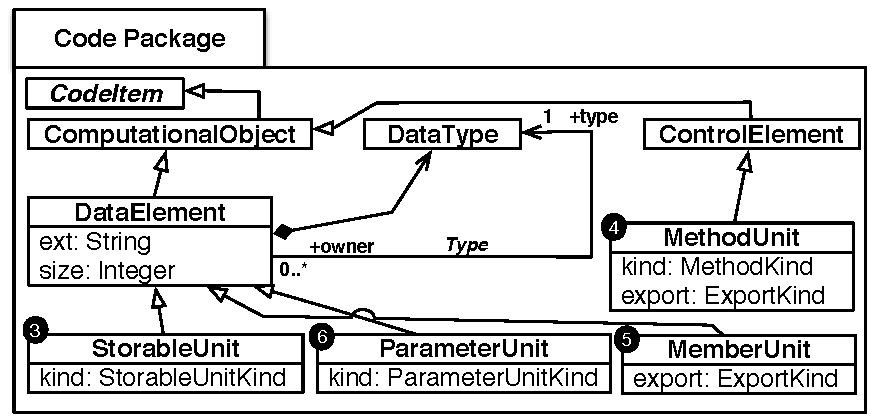
\includegraphics[scale=0.67]{images/StorableUnit_MethodUnit2}
	\label{fig:StorableUnit_MethodUnit}
	\fadaptada{KDM:specification}
\end{figure}


%As stated before, the meta-class \texttt{ClassUnit} represents user-defined classes in object-oriented languages. A class datatype is a named datatype that represents a class: an ordered collection of named elements, each of which can be another \texttt{CodeItem}, such as a \texttt{StorableUnit} or a \texttt{MethodUnit}. The meta-class \texttt{ClassUnit} contains a meta-attribute \texttt{isAbstract:Boolean} used to specify if the class is abstract or not. \texttt{ClassUnit} also has an meta-association named \texttt{codeElement:CodeItem[0..*]} that is used to group all class's members, e.g., fields, constructor, methods, etc. 

%Similarmente, a metaclasse~$\mathtt{InterfaceUnit}$ representa o conceito comum a várias linguagens de programação. Ela é uma subclasse de~$\mathtt{DataType}$, assim como~$\mathtt{ClassUnit}$.~$\mathtt{InterfaceUnit}$ também possui uma meta associação chamada~$\mathtt{codeElement:CodeItem[0..*]}$ que representa tipos de dados tal como~$\mathtt{MethodUnit}$.

%Similarly, the meta-class \texttt{InterfaceUnit} represents the interface concept common to various programming languages. It is also a subclass of \texttt{Datatype} as \texttt{ClassUnit}. \texttt{InterfaceUnit} also has an meta-association named \texttt{codeElement:CodeItem[0..*]} that represent data types as well as \texttt{MethodUnits}.

$\mathtt{StorableUnit}$ representa um atributo em um sistema de software - um objeto computacional para que diferentes valores do mesmo tipo de dados possam ser associados. Ele é usado para representar as variáveis globais e locais. Ele engloba um meta atributo~$\mathtt{String}$ usado para definir o nome das variáveis.~$\mathtt{StorableUnit}$ também tem a associação~$\mathtt{type:DataType[1]}$, a qual é herdada da metaclasse~$\mathtt{DataElement}$, e é utilizado para especificar o tipo da variável (\textit{int, char, boolean, numeric}, etc). Ele também tem uma enumeração ~$\mathtt{kind:StorableUnit}$, que descreve várias propriedades comuns de um ~$\mathtt{StorableUnit}$ relacionado com o seu ciclo de vida, por exemplo, sua visibilidade (\textit{private, public, protected}, etc).

%\texttt{StorableUnit} represents a variable of existing software system - a computational object to which different values of the same datatype can be associated at different times. It is used to represent both global and local variables. It contains a meta-attribute \texttt{name:String} used to set the name of the variables. \texttt{StorableUnit} also has the association \texttt{type:Datatype[1]} used to specify the variable's type. It also has a enumeration \texttt{kind:StorableKind}, it describes several common properties of a \texttt{StorableUnit} related to their life-cycle, visibility, and memory type. 

~$\mathtt{MethodUnit}$, como o próprio nome sugere, representa métodos que são identificados em ~$\mathtt{ClassUnit}$ ou~$\mathtt{InterfaceUnit}$. Também é usado para representar construtores e destrutores. Possui como meta-atributos~$\mathtt{name:String}$,~$\mathtt{kind:MethodKind}$ e ~$\mathtt{export:ExportKind}$. O primeiro é usado para descrever o nome de um método; o segundo é uma enumeração que define especificações adicionais do tipo de método, ou seja, é possível especificar se a instância do método é um construtor, destrutor, ou um método normal; o último representa a visibilidade do método (\textit{private, public, protected}, etc).

%\texttt{MethodUnit} represents member functions owned by either \texttt{ClassUnit} or \texttt{InterfaceUnit}. It is also used to represent user-defined operators, constructors, and destructors. It owns as meta-attributes \texttt{name:String}, \texttt{kind:MethodKind}, and \texttt{export: ExportKind}. The fist one is used to describe to name of a method. The second meta-attribute is an enumeration that defines additional specification of the kind of method, i.e., it is possible to specify if the method's instance is a constructor, destructor, abstract, etc. The last one represents the visibility of the method, i.e., \texttt{public}, \texttt{private}, \texttt{protected}.

A fim de entender como o KDM é utilizado para representar estruturas em um determinado programa, no Código-fonte~\ref{lst:example_kdm_instance} é mostrado um exemplo simplificado escrito em Java. O correspondente KDM, embora simplificado, é apresentado na Figura~\ref{fig:kdm_instance_Java}. Por questões de simplicidade e para facilitar o entendimento, essa figura ilustra a instância do KDM em forma de um diagrama de objetos; é possível notar que tal diagrama representa o código-fonte como uma árvore, na qual cada nó representa uma metaclasses do KDM. Como pode ser visto na Figura~\ref{fig:kdm_instance_Java}, a metaclasse raiz é ~$\mathtt{Segment}$, que é um recipiente para um conjunto significativo de fatos sobre um sistema de software existente. Cada~$\mathtt{Segment}$ pode incluir uma ou mais instâncias de modelos do KDM, como~$\mathtt{CodeModel}$ e~$\mathtt{StructureModel}$.

%In order to fully understand how KDM is used to represent the source code of a specific program, in Listing~\ref{lst:example_kdm_instance} is shown a simplified example in Java. The corresponding, though simplified KDM instance is depicted in Figure~\ref{fig:kdm_instance_Java}. It illustrates a KDM instance as a UML object diagram for the sake of simplicity, note that this diagram represents the source code as a tree of nodes containing some KDM's metaclasses. As can be seen in Figure~\ref{fig:kdm_instance_Java} the root meta-class is \texttt{Segment}, which is a container for a meaningful set of facts about an existing software system. Each \texttt{Segment} may include one or more KDM model instances, such as \texttt{CodeModel} and \texttt{StructureModel}. As stated earlier, the \texttt{CodeModel} is the specific KDM container for other \texttt{code} element instances (see Figure~\ref{fig:CodeModel}). 

\noindent\begin{minipage}{.53\textwidth}
	\begin{codigo}[caption={[Parte de código Java para ilustrar como o KDM é usado para representar o código fonte.] Simples código em Java.},escapeinside={(*@}{@*)}, basicstyle=\footnotesize, label={lst:example_kdm_instance}]{Name}
	(*@\ding{202}@*) package model;
	(*@\ding{203}@*) public class Car (*@\ding{204}@*) extends  
	(*@\ding{205}@*) Vehicle{
	(*@\ding{229}@*)(*@\ding{206}@*) private String name;
	(*@\ding{229}@*)(*@\ding{207}@*) public String getName(){
	(*@\ldots @*)
	}
	}
	\end{codigo}
\end{minipage}\hfill
\begin{minipage}{.45\textwidth}
	\centering
	% Requires \usepackage{graphicx}
	\captionof{figure}{Instância KDM correspondente ao Código-fonte~\ref{lst:example_kdm_instance}.}
	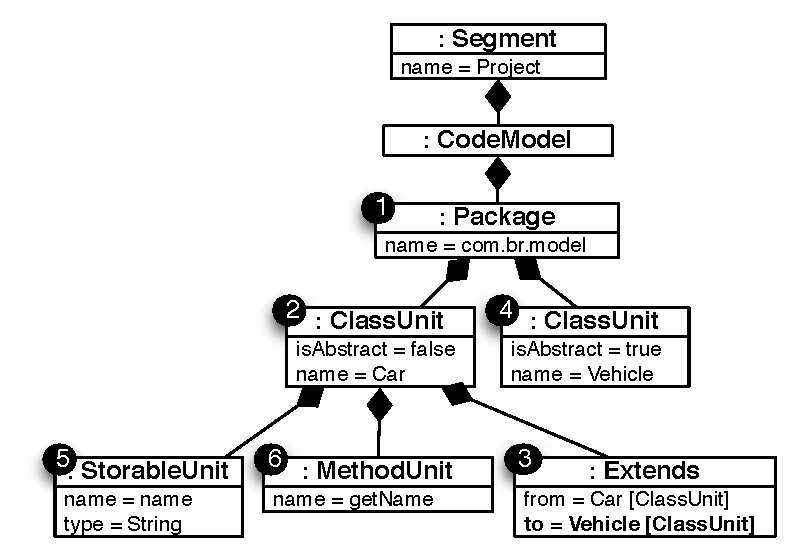
\includegraphics[scale=0.6]{images/kdm_instance_java_correspoding_2_with_extends}
	\fautor
	\label{fig:kdm_instance_Java}
\end{minipage}

Analisando tanto o Código-fonte~\ref{lst:example_kdm_instance}, quanto a Figura~\ref{fig:kdm_instance_Java}, é evidente que cada estrutura estática do código-fonte tem uma metaclasse específica em KDM para representá-la. Por exemplo, a declaração \textit{package} \textit{model} na Linha 1 do Código-fonte~\ref{lst:example_kdm_instance} \ding{202} é representada em KDM pela metaclasse ~$\mathtt{package}$, como visto na Figura~\ref{fig:kdm_instance_Java} \ding{202}. Posteriormente, como apresentado no Código-fonte~\ref{lst:example_kdm_instance} \ding {203} uma classe~$\mathtt{Car}$ é declarada. Essa classe herda características da classe~$\mathtt{Vehicle}$, no Java isso é feito por meio da palavra-chave~$\mathtt{extends}$ seguida do nome de uma classe, conforme observado no Código-fonte~\ref{lst:example_kdm_instance} \ding{204} e \ding{205}. A metaclasse~$\mathtt{Extends}$ representa o conceito de herança em KDM. Como mostrado na Figura~\ref{fig:kdm_instance_Java} \ding {204}, a metaclasse~$\mathtt{Extends}$ possui duas associações,~$\mathtt{to}$ e~$\mathtt{from}$; a primeira representa a classe pai (\textit{super class}), e a última a classe filha(\textit{sub-class}). Neste contexto, a classe~$\mathtt{Car}$ é a classe pai de~$\mathtt{Vehicle}$, como mostrado na Figura~\ref{fig:kdm_instance_Java} \ding{205}. Finalmente, o atributo~$\mathtt{name}$ e o método~$\mathtt{getName()}$ (ver Código-fonte~\ref{lst:example_kdm_instance} \ding {206} e \ding {207}, respectivamente) são mapeados para os correspondentes elementos do KDM,~$\mathtt{StorableUnit}$ e~$\mathtt{MethodUnit}$ (ver Figura ~\ref{fig:kdm_instance_Java} \ding {206} e \ding {207}). 
%
%Analyzing both the Listing~\ref{lst:example_kdm_instance} and the Figure~\ref{fig:kdm_instance_Java} it is evident that each static structure of the source code has a meta-class in KDM to represent it. For instance, the package model in Line 1 of Listing~\ref{lst:example_kdm_instance} \ding{202} is represented in KDM by the meta-class named \texttt{Package}, see Figure~\ref{fig:kdm_instance_Java} \ding{202}. In addition, the class \texttt{Car} is declared, see Listing~\ref{lst:example_kdm_instance} \ding{203}. It also inherit from class \texttt{Vehicle}, in the Java this is accomplished by using the keyword \texttt{extends} following of a class, see Listing~\ref{lst:example_kdm_instance}  \ding{204} and \ding{205}. The meta-class \texttt{Extends} represents inheritance in KDM models. As shown in Figure~\ref{fig:kdm_instance_Java} \ding{204} the meta-class \texttt{Extends} has two association, \texttt{to} and \texttt{from}, the former represents the parent class (super class), and the latter represents the child class (sub-class). In this context, the child is the class \texttt{Car} and the parent class is \texttt{Vehicle}, which is depicted in Figure~\ref{fig:kdm_instance_Java} \ding{205}. Finally, the variable \texttt{name}, and the method \texttt{getName()} (see Listing~\ref{lst:example_kdm_instance} \ding{206}, and \ding{207}) are mapped to corresponding instances of the KDM elements, \texttt{StorableUnit}, and \texttt{MethodUnit} (see Figure~\ref{fig:kdm_instance_Java} \ding{206}, and \ding{207}). 
%
%
%
Apenas metaclasses utilizadas para representar estruturas e construções estáticas foram demonstradas. No entanto, o KDM  abrange um pacote que permite a representação de construções dinâmicas, em outras palavras, o pacote \textit{Action} contém metaclasses, cujas finalidades são  permitir e representar comportamento  com relação à execução. Na seção a seguir, mais informações sobre esse pacote são apresentadas.

\subsection{Pacote Action}\label{sec:actionPackage}

O pacote~$\mathtt{Action}$ define um conjunto de metaclasses, com o propósito de representar descrições de comportamento em nível de implementação estabelecida por linguagens de programação, por exemplo, declarações, operadores, condições e as suas associações. A Figura ~\ref{fig:actionModel} \ding {202} mostra o pacote~$\mathtt{Action}$ e algumas de suas metaclasses. Nota-se que esse pacote estende o pacote~$\mathtt{Code}$ (ver a Figura~\ref {fig:actionModel} \ding {208}).

%The \texttt{Action} package defines a set of metaclasses whose purpose is to represent implementation-level behavior descriptions determined by programming languages, for example statements, operators, conditions, features, as well as their associations, for example control and data flow. The Figure~\ref{fig:actionModel} \ding{202} shows the\texttt{Action} package and some of its metaclasses. As can be observed it extends the KDM \texttt{Code} package (see Figure~\ref{fig:actionModel} \ding{208}). 

\begin{figure}[!ht]
	\centering
	% Requires \usepackage{graphicx}
	\caption{Diagrama de classes ilustrando o pacote~$\mathtt{Action}$.}
	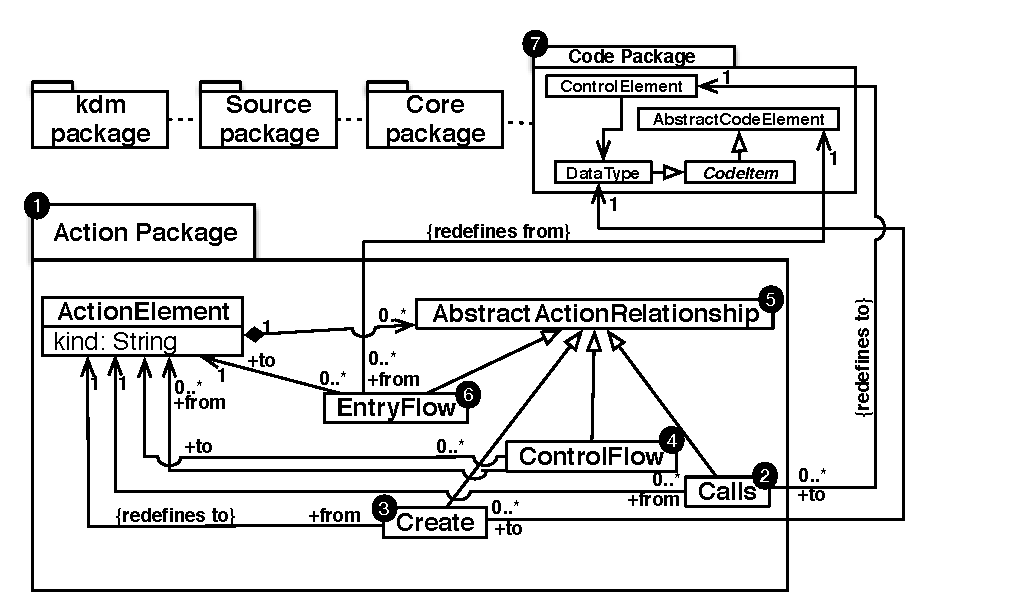
\includegraphics[scale=0.67]{images/ActionModel_Class_Diagram}
	\label{fig:actionModel}
	\fadaptada{KDM:specification}
\end{figure}

O pacote~$\mathtt{Action}$ é composto por 11 diagramas de classes e também depende dos pacotes~$\mathtt{Core}$, ~$\mathtt{kdm}$ e ~$\mathtt{Source}$, e,  principalmente, do pacote~$\mathtt{Code}$. No entanto, o pacote~$\mathtt{Action}$ segue o padrão uniforme para os modelos KDM e estende o KDM com metaclasses específicas relacionadas com o comportamento do nível de implementação. O pacote~$\mathtt{Action}$ se desvia de um padrão uniforme para os modelos KDM porque ele não define um modelo KDM separado, mas estende o pacote~$\mathtt{Code}$.  Por isso, cada metaclasse do pacote ~$\mathtt{Action}$ é uma subclasse de~$\mathtt{AbstractCodeElement}$, conforme destacado na Figura~\ref{fig:actionModel}. O pacote~$\mathtt{Action}$ define a maioria das metaclasses que têm como objetivo representar comportamentos para as construções estáticas definidas no pacote~$\mathtt{Code}$. Assim, ambos os pacotes constituem a CEP, como mostrado na Figura~\ref{fig:kdm_layer}.

%The \texttt{Action} package consists of 11 class diagrams, it also depends on the \texttt{Core}, \texttt{kdm}, \texttt{Source}, and mainly \texttt{Code}. However, the \texttt{Action} package follows the uniform pattern for KDM models and extends the KDM with specific metaclasses related to implementation-level behavior. The \texttt{Action} package deviates from a uniform pattern for KDM models because it does not define a separate KDM model, but rather extends the \texttt{Code}, which is presented in Section~\ref{codePackage}. Therefore each \texttt{Action} metaclasses is a subclass of \texttt{AbstractCodeElement}, as highlighted in Figure~\ref{fig:actionModel}. \texttt{Action} package defines most of the relationship types to the \texttt{Code} model. Together, \texttt{Action}, and \texttt{Code} packages constitute the Program Elements Layer of KDM as depicted in Figure~\ref{fig:all_kdm_layers}. 

A metaclasse~$\mathtt{AbstractionActionRelationship}$ apresentada na Figura~\ref{fig:actionModel} \ding{206} é a metaclasse pai usada para representar várias relações que se originam a partir de um~$\mathtt{ActionElement}$. Além disso, essa metaclasse~$\mathtt{AbstractionActionRelationship}$ possui metaclasses específicas; algumas delas estão representadas na Figura~\ref{fig:actionModel}, por exemplo, as metaclasses~$\mathtt{Calls}$ \ding {203},~$\mathtt{Creates}$ \ding {204},~$\mathtt{ControlFlow}$ \ding {205} e~$\mathtt{EntryFlow}$ \ding{207}.

%The meta-class \texttt{AbstractActionRelationship} presented in Figure~\ref{fig:actionModel} \ding{206} is the parent class used to represent various KDM relationships that originate from an \texttt{ActionElement}. The meta-class \texttt{AbstractActionRelationship} owns specific metaclasses. Some of them are depicted in Figure~\ref{fig:actionModel}, for example, the metaclasses \texttt{Calls} \ding{203}, \texttt{Create} \ding{204}, \texttt{ControlFlow} \ding{205}, and \texttt{EntryFlow} \ding{207}.

O relacionamento~$\mathtt{Calls}$ corresponde a uma chamada para um procedimento, um método estático, um método não-estático de uma instância particular de um objeto, um método virtual, ou um elemento de interface.~$\mathtt{Calls}$ possui duas associações, são elas: ~$\mathtt{ActionElement[1]}$ e ~$\mathtt{ControlElement[1]}$. A primeira representa o elemento de ação a partir do qual a relação chamada origina, e a segunda associação representa o elemento alvo.

%\texttt{Calls} relationship corresponds to ``invoke'' operation on a procedure type. It can represent a call to a procedure, a static method, a non-static method of a particular object instance, a virtual method, or an interface element. \texttt{Calls} has two associations, they are: \texttt{from:ActionElement[1]} and \texttt{to:ControlElement[1]}. The first one represents the action element from which the call relation originates. The second association represents the target \texttt{ControlElement}.

A metaclasse~$\mathtt{Creates}$ representa uma associação entre um elemento de ação que \aspas{cria} uma nova instância de um determinado elemento de dados. Por exemplo, em Java, essa metaclasse corresponde à palavra-chave \texttt{new}, utilizada para instanciar um novo objeto. $\mathtt{Creates}$ também possui duas associações:~$\mathtt{ActionElement[1]}$ e~$\mathtt{DataType[1]}$. Similar a metaclasse~$\mathtt{Calls}$, a primeira associação representa o elemento que possui o relacionamento e a segunda representa o elemento de dados (objeto), que é instanciado pelo~$\mathtt{ActionElement}$.

%The meta-class \texttt{Create} represents an association between an action element that ``creates'' a new instance of a certain data element to the corresponding datatype according to the semantics of the programming language of the existing software system. It also has association, \texttt{from:ActionElement[1]} and \texttt{to:Datatype[1]}. Similarly, to the meta-class \texttt{Calls}, the first association represents the element that owns the \texttt{Creates} relationship. The second one illustrates the \texttt{DataElement} that is instantiated by the \texttt{ActionElement}. 

O~$\mathtt{ControlFlow}$ é um elemento de modelagem genérica que representa relação de fluxo de controle entre dois~$\mathtt{ActionElements}$. Além disso, é uma submetaclasse com elementos de modelagens mais específicas. O~$\mathtt{EntryFlow}$ é um elemento de modelagem que representa um fluxo inicial de controle em um elemento KDM. O relacionamento~$\mathtt{EntryFlow}$ é usado de uma maneira uniforme para descrever os pontos de entrada para outros elementos de código KDM.

%The \texttt{ControlFlow} is a generic modeling element that represents control flow relation between two \texttt{ActionElements}. It is further subclassed with more specific modeling elements. The \texttt{EntryFlow} is a modeling element that represents an initial flow of control into a KDM element. The \texttt{EntryFlow} relationship is used in a uniform way for describing entry points to other KDM code elements. 



A fim de compreender como o pacote~$\mathtt{Action}$ é usado no KDM, no Código-fonte~\ref{lst:example_kdm_instance_2} é mostrado um simples método implementado em Java. Nesse método é criada uma instância de~$\mathtt{Car}$ e seu método de acesso é invocado. Uma possível correspondente instância do KDM simplificada é apresentada na Figura~\ref{fig:kdm_instance_Java_action}. Nota-se que o diamante em destaque na cor cinza e anexado com três pontos (\ldots) ilustra que outras metaclasses não são mostradas com o intuito de simplificar a figura.

%In order to comprehend  how the \texttt{Action} package is used in KDM, in Listing~\ref{lst:example_kdm_instance_2} shows a simple method implemented in Java. In this method is created an instance of \texttt{Car} and an accessor method of it is called, ie., the \texttt{getName()}. The corresponding simplified KDM instance is depicted in Figure~\ref{fig:kdm_instance_Java_action}. Please note that, the diamond highlighted in grey and attached with three dots (\ldots) illustrates that other metaclasses are not shown in order to simplify the figure.  

\noindent\begin{minipage}{.43\textwidth}
	\begin{codigo}[caption={[Pedaço de código Java para ilustrar como o pacote~$\mathtt{Action}$ funciona.] Método \texttt{e1} ilustrando como o Pacote \texttt{Action} funciona.}, escapeinside={(*@}{@*)}, basicstyle=\footnotesize, label={lst:example_kdm_instance_2}]{Name}
	(*@\ldots @*)
	public void e1 (*@\ding{202}@*)(){
	Car myCar (*@\ding{203}@*) = new Car() (*@\ding{204}@*);
	(*@\ding{229}@*)myCar.getName() (*@\ding{205}@*);
	}
	(*@\ldots @*)
	\end{codigo}
\end{minipage}\hfill
\begin{minipage}{.65\textwidth}
	\centering
	\captionof{figure}{Instância KDM correspondente ao Código-fonte~\ref{lst:example_kdm_instance_2}.}
	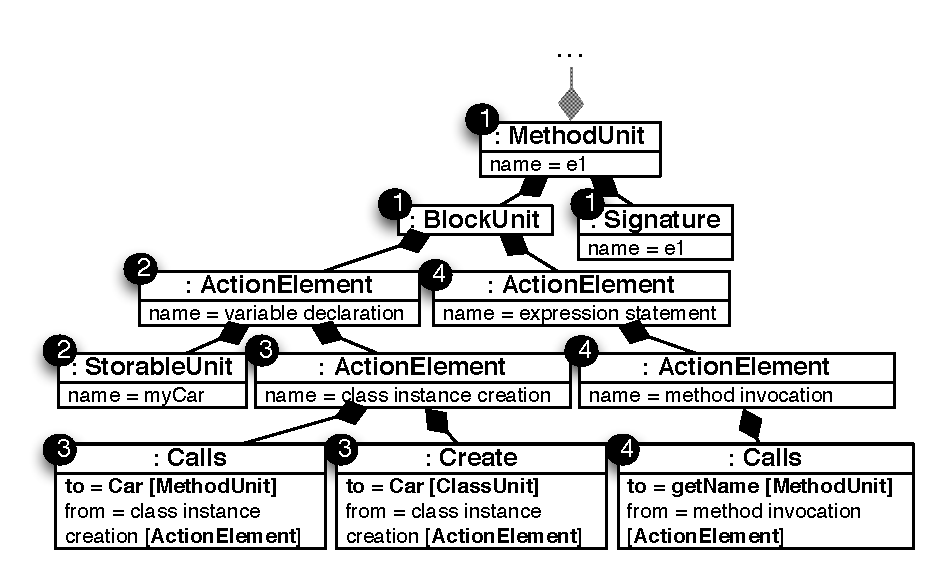
\includegraphics[scale=0.6]{images/actionInstanceKDM_2}
	\fautor
	\label{fig:kdm_instance_Java_action}
\end{minipage}


As três primeiras metaclasses mostradas nessa hierarquia são~$\mathtt{MethodUnit}$,~$\mathtt{BlockUnit}$ e~$\mathtt{Signature}$ conforme destacado na  Figura~\ref{fig:kdm_instance_Java_action} \ding{202}. Essas três metaclasses basicamente representam uma declaração e a assinatura de um determinado método, no caso \texttt{e1()}. Mais especificamente, a metaclasse~$\mathtt{MethodUnit}$ é usada para representar o método~$\mathtt{e1()}$ como mostrado tanto no Código-fonte~\ref{lst:example_kdm_instance_2} \ding{202}, quanto na Figura~\ref{fig:kdm_instance_Java_action} \ding{202}.~$\mathtt{BlockUnit}$ representa blocos lógicos e físicos relacionados a~$\mathtt{ActionElement}$, ou seja, o escopo do método representado por \{...\}. Por sua vez,~$\mathtt{Signature}$ representa a assinatura do método, isto é, essa metaclasse representa além do nome do método todos os parâmetros, o retorno do método, exceções, etc.	

%The first three metaclasses shown in this hierarchy are the \texttt{MethodUnit}, \texttt{BlockUnit}, and \texttt{Signature} (see Figure~\ref{fig:kdm_instance_Java_action} \ding{202}). These metaclasses are used to represent a simple method declaration. More specifically, the meta-class \texttt{MethodUnit} is used to represent the method \texttt{e1} as shown in both Listing~\ref{lst:example_kdm_instance_2} \ding{202} and Figure~\ref{fig:kdm_instance_Java_action} \ding{202}. \texttt{BlockUnit} represents logically and physically related blocks of \texttt{ActionElement}, i.e., the area between the braces, \texttt{\{\ldots\}}. In turn, \texttt{Signature} represents the concept of a method signature, i.e., it also can be used to represent the name of the method, all the parameters, the return of the method, etc.

Na Linha 12 do Código-fonte~\ref{lst:example_kdm_instance_2} \ding{203}, uma variável chamada~$\mathtt{myCar}$ é declarada. As metaclasses que representam essa declaração podem ser visualizadas na Figura~\ref{fig:kdm_instance_Java_action} \ding{203}. A metaclasse~$\mathtt{ActionElement}$ representa o significado das operações, por exemplo, uma declaração da variável. A metaclasse~$\mathtt{StorableUnit}$ representa a própria variável \texttt{myCar}. Ainda na Linha 10 \ding{204}, a instância da classe~$\mathtt{Car}$ é criada usando a palavra-chave~$\mathtt{new}$. Nota-se que na Figura~\ref{fig:kdm_instance_Java_action} \ding{204} três metaclasses são utilizadas para representar o operador~$\mathtt{new}$. Primeiramente, a metaclasse~$\mathtt{ActionElement}$ é usada para ilustrar o significado da operação, nesse caso, a instância da classe \texttt{Car}. A metaclasse~$\mathtt{Calls}$ é usada para ilustrar a instanciação de um objeto, nesse caso, o objeto~$\mathtt{Car}$. Adicionalmente, a metaclasse \texttt{Calls} posssui duas associações: ~$\mathtt{to}$ e~$\mathtt{from}$, as quais representam a chamada para o construtor de~$\mathtt{Car}$ e representam o alvo~$\mathtt{ActionElement}$, respectivamente. Em seguida, a metaclasse~$\mathtt{Creates}$ representa a nova instância de~$\mathtt{Car}$.

%In Line 10 of the Listening~\ref{lst:example_kdm_instance_2} \ding{203} a variable named \texttt{myCar} is declared. The corresponding metaclasses representing this variable declaration can be visualized in Figure~\ref{fig:kdm_instance_Java_action} \ding{203}. The meta-class \texttt{ActionElement} represents the meaning of the operations, i.e., ``variable declaration''. The \texttt{StorableUnit} represents the variable itself. Still in Line 10 \ding{204} the instance of the class \texttt{Car} is created by using the keyword \texttt{new}. Note that in Figure~\ref{fig:kdm_instance_Java_action} \ding{204} three metaclasses are used to illustrate the operator \texttt{new}. Firstly, the meta-class \texttt{ActionElement} is used to illustrate the meaning of the operation, in this case ``class instance creation'' . Secondly, the meta-class \texttt{Calls} is used to illustrate the instantiation of an object, herein \texttt{Car} object. Its owns two association, i.e., \texttt{to} and \texttt{from} which illustrates the call to the constructor of \texttt{Car} and represents the target \texttt{ActionElement}, respectively. Thirdly, the meta-class \texttt{Creates} represents the new instance of the \texttt{Car}.

Na linha 11 do Código-fonte~\ref{lst:example_kdm_instance_2} \ding{205}, um método acessor é invocado. Como pode ser visto na Figura~\ref{fig:kdm_instance_Java_action} \ding{205}, três metaclasses são utilizadas no KDM para representar essa linha. Primeiro é criada uma metaclasse~$\mathtt{ActionElement}$ que representa a declaração em si. Em seguida, outro~$\mathtt{ActionElement}$ é criado para representar a invocação de método. Finalmente, outra metaclasse~$\mathtt{Calls}$ é instanciada para representar a chamada do método~$\mathtt{getName()}$.

\subsection{Pacote \textit{Structure}}\label{sec:structurePackage}

O KDM define metaclasses que representam componentes arquiteturais, como subsistemas, camadas, componentes, etc., e define também a rastreabilidade desses elementos para outras metaclasses do KDM para o mesmo sistema por meio do pacote \texttt{Structure}.

\begin{figure}[h]
	\centering
	% Requires \usepackage{graphicx}
	\caption{Diagrama de classes do pacote \texttt{Structure}\label{fig:structureModel}}
	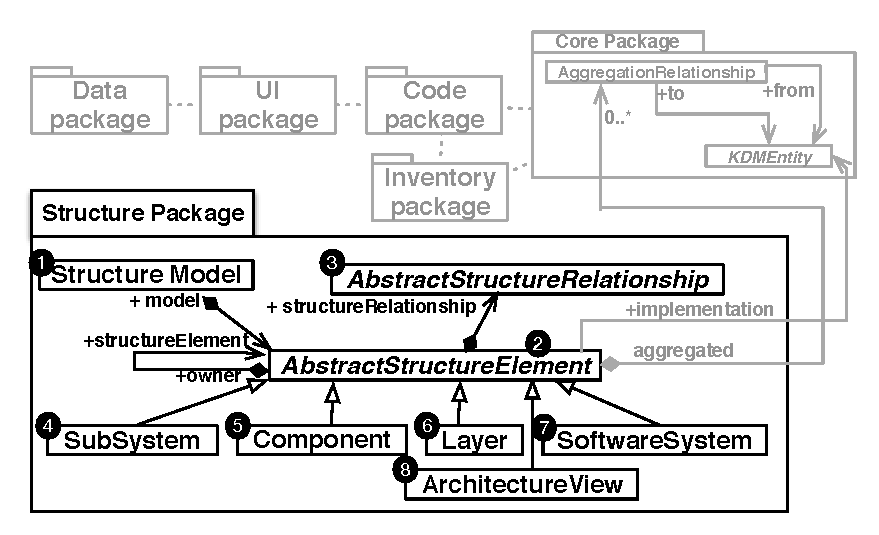
\includegraphics[scale=0.67]{images/StructurePackageFigure}
	\fadaptada{ADM:OMG}
\end{figure}

Esse pacote define um ponto de vista arquitetural para um domínio estrutural. As visões de arquitetura com bae no ponto de vista definido pelo pacote \texttt{Strcuture} representam a forma como os elementos estruturais do sistema de software estão relacionados como os módulos definidos em código-fonte, que correspondem ao pacote \texttt{Code} do KDM. Uma parte simplória do pacote \texttt{Structure} é apresentada na Figura~\ref{fig:structureModel} como um diagrama de classes.

 Usando suas metaclasses é possível relacionar todos os elementos estruturais do sistema, juntamente com os elementos computacionais, isto é, pode-se especificar os elementos estruturais do sistema. Na Figura~\ref{fig:structureModel} é mostrado que o pacote \texttt{Structure} e suas metaclasses são usadas em combinação com os pacotes \texttt{Code}, \texttt{Data}, \texttt{Platform}, \texttt{UI} e \texttt{Inventory}. O modelo \texttt{Structure} possui uma coleção de elementos estruturais, como pode ser visto na Figura~\ref{fig:structureModel} \ding{202}, isso é representado por meio de uma associação. Pacotes (do modelo \texttt{Code}) são os elementos folha do modelo \texttt{Structure}, representando a divisão de um sistema em módulos \texttt{Code} discretos, com partes não sobrepostas. A metaclasse \texttt{SoftwareSystem} fornece um ponto de encontro para todos os pacotes do sistema direta ou indiretamente através de outra associação chamada de \texttt{AbstractStructureElement[0..*]}. Os pacotes podem ainda ser agrupados nas metaclasses \texttt{SubSystem},\texttt{Layer},\texttt{Component} e \texttt{ArchitectureView}. 
 
A metaclasse \texttt{AbstractStructureElement} (conforme a Figura~\ref{fig:structureModel} \ding {203}) representa uma parte arquitetural, relacionada com a organização do sistema de software existente em módulos e possui quatro associações. A primeira associação representa os elementos pertencentes ao modelo e é chamada de $\mathtt{structureElement}$ $\mathtt{:AbstractStructureElement[0..*]}$. Em seguida, há a associação~$\mathtt{structureRelationship}$ $\mathtt{:AbstractStructureRelationship[0..*]}$, ela é usada para representar todas os relacionamentos em nível arquitetural. A associação $\mathtt{aggregated:}$ $\mathtt{AggregatedRelationship[0..*]}$ representa uma relação abstrata entre dois elementos do KDM, dentro dela é possível definir relações concretas. A última associação da metaclasse~$\mathtt{AbstractStructureElement}$ é o~$\mathtt{implementation:KDMEntity[0..*]}$. Esta associação é usada para especificar os elementos computacionais (do pacote~$\mathtt{Code}$, ou seja, $\mathtt{Package}$, $\mathtt{ClassUnit}$, $\mathtt{InterfaceUnit}$, etc) que representam o elemento estrutural. 

Na Figura~\ref{fig:kdm_structureExample} é descrita uma possível arquitetura mostrada para ilustrar como o KDM pode ser utilizado para representar elementos arquiteturais. Pode ser observado que esta figura é dividida em três níveis para ilustrar como o pacote~$\mathtt{Structure}$ está relacionado com o pacote~$\mathtt{Code}$. O nível mais baixo representa o código-fonte, artefatos físicos. L1 e L2 representam pacotes em código-fonte - cada caixa dentro dos pacotes representa as suas classes e interfaces, também é possível perceber que essas classes e interfaces são relacionados uns com os outros de alguma maneira. No meio há metaclasses do pacote~$\mathtt{Code}$, o que significa que as instâncias dessas meta -classes são usadas para representar os artefatos de baixo nível, ou seja, instâncias de~$\mathtt{Package}$ são usadas para representar L1 e L2 e instâncias de~$\mathtt{ClassUnit}$ e~$\mathtt{InterfaceUnit}$ são usados para representar as classes e interfaces, respectivamente. Finalmente, no nível superior a arquitetura é mostrada. Todos os elementos arquiteturais são representados com a seguinte padronização: a metaclasse que representa o elemento arquiteturais, ':' seguido pelo seu nome. A arquitetura apresentada é dividida da seguinte forma: no ponto mais alto de abstração há um~$\mathtt{SoftwareSystem}$ ($\mathtt{S1}$) \ding {202}, que é dividido em duas camadas, ~$\mathtt{Layer}$~$\mathtt{L1}$ \ding {203} e ~$\mathtt{Layer}$~$\mathtt{L2}$ \ding {204}. Tais camadas representam elementos arquiteturais correspondentes aos pacotes L1 e L2 representadas no nível mais baixo. A~$\mathtt{Layer}$~$\mathtt{L1}$ pode acessar os elementos da~$\mathtt{Layer}$~$\mathtt{L2}$, essa restrição \aspas{pode acessar} é representada pela metaclasse~$\mathtt{AggregatedRelationship}$ \ding {205}. Além disso, a~$\mathtt{Layer}$~$\mathtt{L2}$ contém dois componentes,~$\mathtt{C1}$ \ding {206} e~$\mathtt{C2}$ \ding {207}. Finalmente, o~$\mathtt{Component}$~$\mathtt{C1}$ fornece recursos através de uma interface para o~$\mathtt{Component}$~$\mathtt{C2}$.

\noindent \begin{minipage}{.47\textwidth}
	\centering
	\captionof{figure}{Exemplo de uma Arquitetura.}
	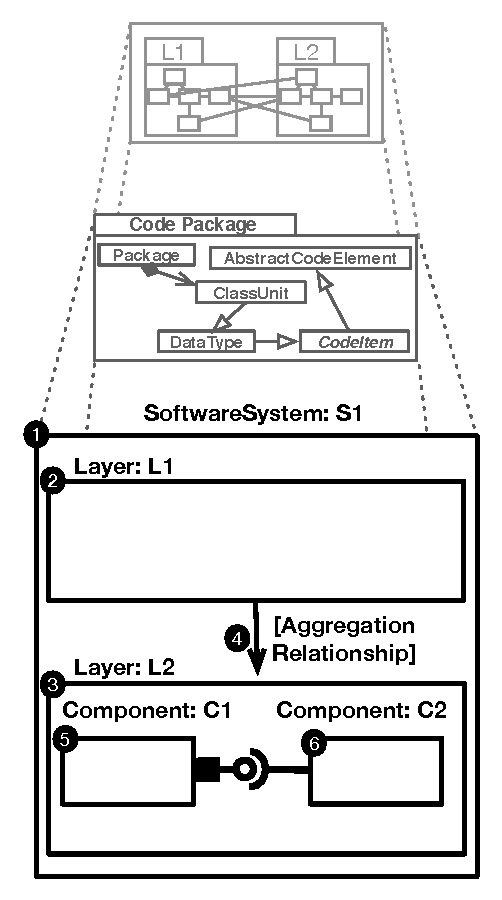
\includegraphics[scale=0.7]{images/StructureExample}
	\fautor
	\label{fig:kdm_structureExample}
\end{minipage}\hfill
\begin{minipage}{.55\textwidth}
	\centering
	\captionof{figure}{Instância KDM correspondente à Figura~\ref{fig:kdm_structureExample}}
	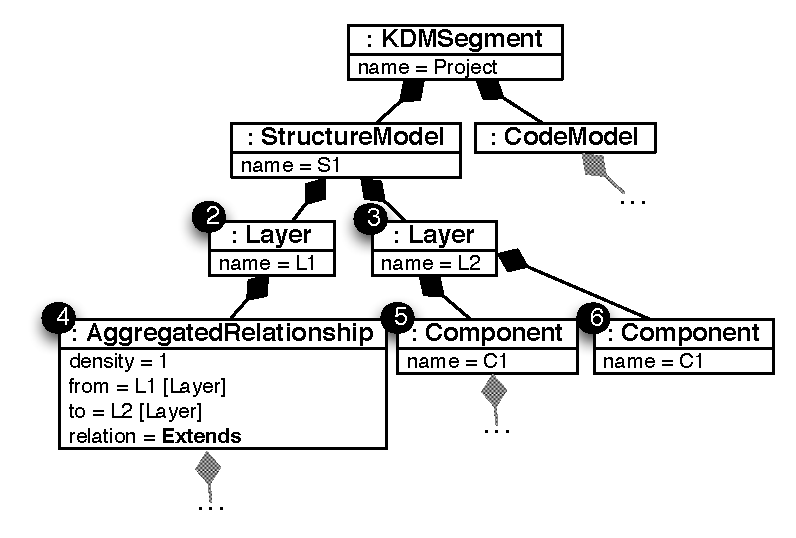
\includegraphics[scale=0.67]{images/StructureKDMINstance}
	\fautor
	\label{fig:kdm_instance_StructureExample}
\end{minipage}


O correspondente, porém simplificado da instância KDM é mostrado na Figura~\ref{fig:kdm_instance_StructureExample}. Os diamantes destacadas em cinza e em anexo com três pontos (\ldots) ilustram que algumas metaclasses não são mostrados de forma a simplificar a figura. Todos os elementos arquiteturais são subclasses de~$\mathtt{StructureModel}$. As camadas são representados pela metaclasse~$\mathtt{Layer}$, como pode ser visto na Figura~\ref{fig:kdm_instance_StructureExample} \ding{203} e \ding{204}. Da mesma forma, os componentes são representados pela metaclasse~$\mathtt{Component}$. A metaclasse mais importante a se destacar nesta figura é $\mathtt{AggregatedRelationship}$. Ela representa a relação entre a $\mathtt{Layer}$ $\mathtt{L1}$ e a $\mathtt{Layer}$ $\mathtt{L2}$. Ela possui meta atributos que tem como objetivo fornecer informações sobre o relacionamento. Por exemplo, o meta atributo~$\mathtt{density}$ ilustra o número de relações primitivas entre estas camadas. Na Figura~\ref{fig:kdm_instance_StructureExample}, o meta atributo~$\mathtt{density}$ possui o valor 1 (um). Outros dois meta atributos são o~$\mathtt{from}$ e o~$\mathtt{to}$, que representam os elementos arquiteturais de origem e destino, respectivamente. Eles são usados para especificar que a~$\mathtt{Layer}$~$\mathtt{L1}$ em~$\mathtt{SoftwareSystem}$~$\mathtt{S1}$ pode acessar a~$\mathtt{Layer}$~$\mathtt{L2}$ também em~$\mathtt{SoftwareSystem}$~$\mathtt{S1}$ de alguma forma. Finalmente, o meta atributo~$\mathtt{relation}$ representa como a~$\mathtt{Layer}$~$\mathtt{L1}$ pode acessar a~$\mathtt{Layer}$~$\mathtt{L2}$, neste contexto, através de herança usando a metaclasse~$\mathtt{Extends}$. Na Figura~\ref{fig:relationship_example_1} é mostrado como as relações entre dois elementos arquiteturais são considerados neste estudo.

\begin{figure}[!ht]
	\centering
	\caption{Relacionamento entre dois elementos arquiteturais}
	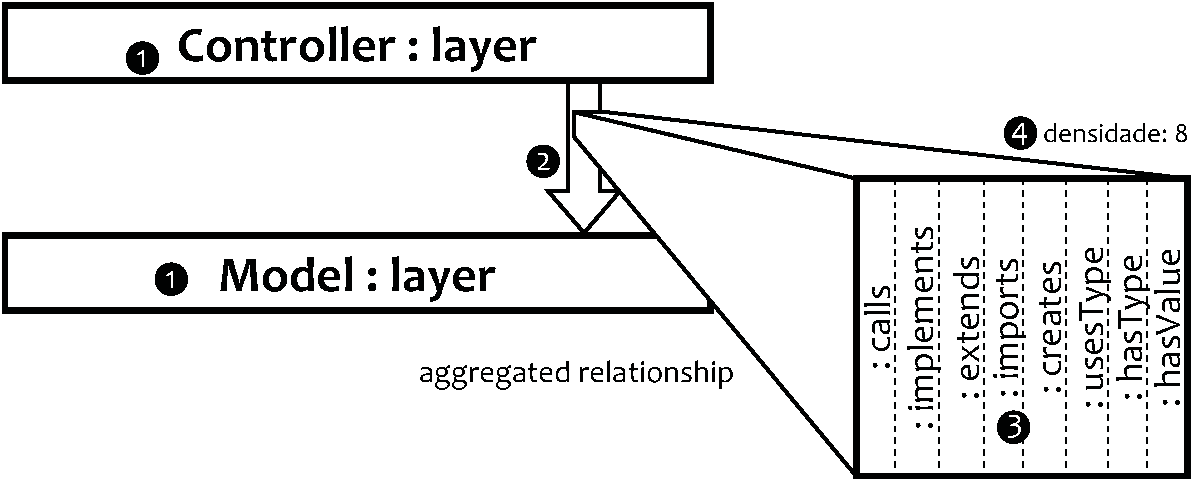
\includegraphics[width=3.3in]{images/relationshipExample1.pdf}
	\fautor
	\label{fig:relationship_example_1}
\end{figure}


Em \ding{202} os elementos arquiteturais são apresentados, camadas~$\mathtt{Controller}$ e~$\mathtt{Model}$. Como visto anteriormente, um relacionamento em nível arquitetural acontece entre dois elementos em nível estrutural (camadas, componentes, subsistemas, etc). Por exemplo, em \ding{203} é mostrando um~$\mathtt{aggregatedRelationship}$ contendo todos os possíveis relacionamentos \ding{204} entre dois elementos (chamadas de métodos, herança, etc). A seta \ding{206} representa o fluxo de entrada e saída dos relacionamentos, em outras palavras, esses relacionamentos representam as possíveis restrições iniciando na camada~$\mathtt{Controller}$  para a camada~$\mathtt{Model}$. Finalmente, a densidade \ding{205} é setada como oito, que representa o número total de relacionamentos possíveis.


\section{Ferramenta de apoio ao KDM}\label{sec:Ferramenta_de_apoio_KDM_capitulo}

Um dos trabalhos mais importantes publicados no contexto da ADM é o de~\citeonline{Bruneliere_2010MODISCO, Bruneliere_2014} que propõe uma ferramenta chamada MoDisco. MoDisco é uma framework genérico e extensível para a abordagem de Engenheria Reversa dirigida a modelos e foi implementada no \sigla{IDE}{\textit{Integrated Development Environment}} Eclipse como um \textit{plug-in}. Mais especificadamente, MoDisco é construido utilizando o \textit{Eclipse Modeling Framework} (EMF). Basicamente essa ferramenta é capaz de recuperar o código-fonte legado, base de dados e outros artefatos legado e representá-los com o metamodelo KDM. Um dos principais objetivos da ferramenta MoDisco é ser adaptável para diferentes cenários, facilitando assim a sua utilização por uma base de usuários potencialmente maior~\cite{Bruneliere_2014}. Inicialmente criado como um modelo experimental de investigação pela Equipe AtlanMod (\sigla{EMN}{\textit{Ecole des mines de Nantes}} \& \sigla{INRIA}{\textit{Institut National de Recherche en Informatique et en Automatique}}), o projeto evoluiu para uma solução industrializados graças à colaboração com a empresa MIA-Software. Este trabalho conjunto ativo resultou em um conjunto eficiente e utilizável de ferramentas para a descoberta, consulta e manipulação de modelos de software para auxiliar toda a atividade de engenharia reversa.

MoDisco tem como objetivo representar uma grande variedade de artefatos (por exemplo, código-fonte, banco de dados, arquivos de configuração, documentação, etc.) de um sistema legado. Contudo, uma das limitações dessa ferramenta é o suporte e a aplicação de refatorações. Observe que, naturalmente, MoDisco não é capaz de aplicar refatorações de forma automática, pois a maioria das refatorações necessitam de interação do usuário para fornecer as informações necessárias. No contexto desta Tese foi utilizado a ferramenta MoDisco para recuperar as informações do código-fonte legado escrito em Java. Sem o auxílio dessa ferramenta todo o sistema legado, escrito em Java, deveria ser transformada em uma instância do KDM de forma manual, o que poderia atrasar esta pesquisa, uma vez que toda a manipulação do KDM foi possível por causa da existência do MoDisco e do seu suporte em Java para manipular o metamodelo KDM. Por exemplo, não é possível para o MoDisco adivinhar quais refatorações devem ser aplicadas e em quais elementos; tais informações devem ser fornecidas por um usuário.


%\begin{figure}[!ht]
%	\centering
%	\caption{Visão geral de um projeto MoDisco.}
%	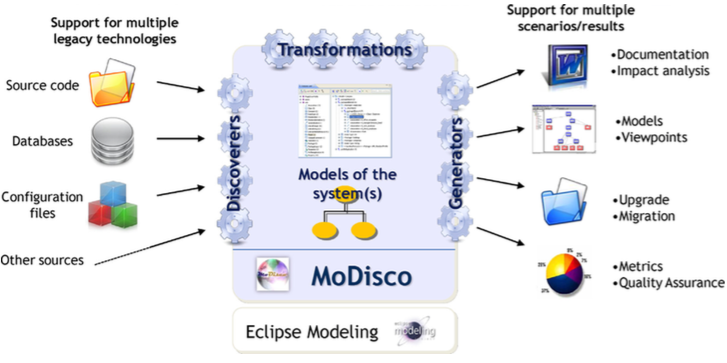
\includegraphics[scale=0.55]{images/modiscoAllArtefacts.png}
%	\label{fig:modisco_allArtefacts}
%	\fadaptada{Bruneliere_2014}
%\end{figure}


\section{Considerações Finais}\label{capitulobaclCOnsideracoesFinais}

Neste capítulo foi apresentada uma revisão dos principais conceitos envolvendo engenharia dirigida por modelos, refatoração, ADM e KDM que são relevantes para a proposta desta Tese. 

Foram discutidas e apresentadas todas as etapas que devem ser realizadas para a condução da engenharia dirigida por modelos, ou seja, todos os níveis CIM, PIM e PSM foram apresentados. Em seguida, foi apresentada a definição e diferença de metametamodelo, metamodelo, modelo e dados. Posteriormente, transformações em modelos foram apresentadas e discutidas, salientando as principais classificações relacionadas a transformações encontradas na literatura - vertical ou horizontal; endógenas ou exógenas. Ainda em relação à transformação de modelos, algumas das principais linguagens utilizadas para realizar a transformação em modelos também foram apresentadas. Porém, apenas a linguagem ATL foi discutida com maiores informações. Os principais conceitos relacionados com refatoração também foram apresentados.


Além disso, este capítulo direciona-se à análise do panorama atual da literatura que trata sobre a modernização de sistemas legados levando em consideração a padronização proposta pelo OMG. Assim, foram mostrados os principais conceitos sobre ADM, KDM, bem como seus pacotes e camadas que são necessários para facilitar o entendimento dessa Tese e também são fundamentais para o desenvolvimento da proposta aqui desenvolvida.

Observou-se também que o metamodelo KDM por intermédio de suas camadas, pacotes e metaclasses permite a criação de um modelo independente de plataforma que representam um sistema em diversas visões. O objetivo do OMG ao criar esse metamodelo é propor uma padronização da reengenharia de software, fornecendo abstrações que ajudem no processo de reengenharia de sistemas. Além disso, pode-se constatar que diferentemente de metamodelos existentes, tais como a UML, o KDM tem como intuito agrupar todos os artefatos (visões) do sistema em um único metamodelo. Dessa forma, pode-se argumentar que o metamodelo KDM pode ser considerado como uma família de metamodelos, uma vez que o mesmo compartilha uma terminologia consistente e homogenia.

Finalmente, este capítulo também apresentou MoDisco, uma das principais ferramentas que automatiza a instanciação do metamodelo KDM. Essa ferramenta foi utilizada no contexto deste trabalho para dar suporte à recuperação de instâncias do metamodelo KDM a partir de código-fonte escrito em Java. No próximo capítulo é apresentado um mapeamento sistemático sobre ADM e KDM que foi conduzido para identificar possíveis desertos de evidências.
